%%%%%%%%%%%%%%%%%%%%%%%%%%%%%%%%%%%%%%%%%%%%%%%%%%

% Latex Kapitel erstellen. 
% 		Kopiere 'texPandoc/*.tex' nach 'content/tex' 
% 		'content/tex' **Handarbeit... für opt. Ergebnisse!** 
% 		Kopiere 'archiv/inhalt.tex' nach 'content/' 
% 		make -- Latex-PDF erstellen 
% ju 28-5-22 inhalt.tex

%%%%%%%%%%%%%%%%%%%%%%%%%%%%%%%%%%%%%%%%%%%%%%%%%%

\chapter{Grundlagen Verbrennungsmotor}
%ju 28-Mai-22 01-Grundlagen-Verbrennungsmotor.tex
\section{Motorbauformen}\label{motorbauformen}

\begin{itemize}
\item
  Reihenmotor, V-Motor, VR-Motor, Boxermotor
\item
  Hubkolbenmotor, Kreiskolbenmotor
\end{itemize}

\section{Hubraum - Brennraum -
Verdichtungsraum}\label{hubraum-brennraum-verdichtungsraum}

$\text{Hubraum} \, V_h = \frac{\pi \cdot d^2}{4} \cdot s \,[cm^3]$

$\text{Gesamthubraum} \, V_H = V_h \cdot z$

$\text{Brennraum} = V_h + V_c$

$\text{Verdichtungsraum} \, V_c = \frac{V_h}{\epsilon - 1}$

$\text{Verdichtungsverhältnis} \, \epsilon = \frac{V_h + V_c}{V_c}$

\section{Arbeitsweise}\label{arbeitsweise}

\begin{enumerate}
\def\labelenumi{(\arabic{enumi})}
\item
  Vier-Takt-Arbeitsverfahren (1 Arbeitsspiel = 2 Kurbelwellenumdrehungen
  = 4 Kolbenhübe)
\item
  Zwei-Takt-Arbeitsverfahren (1 Arbeitsspiel = 1 Kurbelwellenumdrehung =
  2 Kolbenhübe)
\end{enumerate}

\section{Ansaugen}\label{ansaugen}

\begin{itemize}
\item
  Abwärtsgehen des Kolbens
\item
  Volumenvergrößerung, Druckdifferenz (Zylinderdruck versus höhere
  Außendruck)
\item
  Einströmen der Luft (Ansaugen der Luft)
\item
  zündfähiges Kraftstoff-Luft-Gemisch innen/außen bilden (Zylinder,
  Ansaugrohr)
\item
  Kraftstoff (Kohlenstoff -- Wasserstoff - Verbindung)
\end{itemize}

\subsection{Luftdruck}\label{luftdruck}

Luftdruck in Abhängigkeit der geodätischen Höhe

Luftdruck bezogen auf Meereshöhe $(1013~hPa = 1013~mbar, ca.\,1~bar)$

Erdanziehung ist von der Masse abhängig

Das Gewicht der Umgebungsluft drückt auf die Erdoberfläche und erzeugt
einen Druck, Atmosphärendruck.

\subsection{Absolutdruck}\label{absolutdruck}

Druck gegenüber Null (Vakuum, luftleeren Raum)

\subsection{Relativer Druck}\label{relativer-druck}

Druck messen gegenüber Absolutdruck

\subsection{Zusammensetzung der Luft
(Prüfung)}\label{zusammensetzung-der-luft-pruefung}

\begin{itemize}
\item
  $78~\%$ Stickstoff
\item
  $21~\%$ Sauerstoff
\item
  $0,9~\%$ Edelgase
\item
  $0,1~\%$ Partikel, Feinstaub (Zell Gängigkeit, Blutkreislauf,
  Erbgutveränderung > Mutation)
\item
  $0,040~\% ~ CO_2$
\end{itemize}

\section{Verdichten}\label{verdichten}

\begin{itemize}
\item
  Aufwärtsgehen des Kolbens
\item
  Kraftstoff-Luft-Gemisch wird verdichtet
\end{itemize}

\subsection{Hoch verdichtete Motoren}\label{hoch-verdichtete-motoren}

$10:1$

\subsection{Verdichtungsverhältnis}\label{verdichtungsverhaeltnis}

\begin{itemize}
\item
  \textbf{Mazda Motor:} $14:1$
\item
  \textbf{Turbo Motor:} $7 - 8:1$
\item
  \textbf{Direkt:} $17 - 18:1$
\item
  \textbf{Indirekt} (Wirbel, Vorkammer): $21 - 36:1$

  \begin{itemize}
  \item
    Vorkammer > Kugel > Wärmeabgabe
    > höher Verdichten
  \end{itemize}
\end{itemize}

\subsection{Wärme}\label{waerme}

entsteht durch Reibung, Form von Energie, Bewegungsenergie kleiner
Teilchen

\subsection{Wärmeabführung}\label{waermeabfuehrung}

an der Oberfläche, Luft (Isolator)

\subsection{Verdichten z.~B. 10:1}\label{verdichten-z.-b.-101}

$10~l$ großes Volumen wird auf den zehnten Teil verkleinert, also
$1~l$

maximales Volumen zu minimales Volumen

Vgl. >>\emph{Kapitel Rechenbeispiele / Motor - Hubraum - Verdichtung}<<

\subsection{Verdichtungsendtemperatur}\label{verdichtungsendtemperatur}

$600 - 900^\circ\text{C}$ (Diesel: Zündung wird eingeleitet)

\subsection{Entzündungstemperatur
Diesel}\label{entzuendungstemperatur-diesel}

$230 - 250^\circ\text{C}$

\subsection{Zündverzug}\label{zuendverzug}

$Entflammungsphase: \frac{1}{1000} s$

Ziel: Vollständige Verbrennung (feine Zerstäubung und hohe Temperaturen,
das muss schnell gehen)

\begin{enumerate}
\def\labelenumi{(\arabic{enumi})}
\item
  \textbf{Benzin} Beginn Zündfunken bis zur Verbrennung
\item
  \textbf{Diesel} Beginn des Einspritzens bis zur Verbrennung
\end{enumerate}

\subsection{Thermodynamischer Kreisprozess (keine
Prüfung)}\label{thermodynamischer-kreisprozess-keine-pruefung}

Wärmekraftmaschine: Verhältnis von Druck, Volumen und Temperatur beim
Verdichten

Verhindert man die Ausdehnung, z.~B. beim Verdichten, so verdoppelt sich
der Druck.

Pro Grad der Erwärmung steigt der Druck um 273sten Teil seines Volumens
im geschlossenen System

Erwärmt man das Gas um $273~K$, so dehnt es sich auf das doppelte
Volumen aus. Die Temperatur steigt und damit der Druck.

Grundlage: \textbf{1. Satz der Thermodynamik} >>Die Energie bleibt in
einem geschlossenen System konstant.<<

\textbf{Faktor 2} $\Rightarrow \frac{546}{273}$

Ziel: von $20^\circ\text{C} \Rightarrow 600^\circ\text{C}$
Verdichtungsendtemperatur

z.~B. Verdichtung: $(10:1)$ $1~bar \Rightarrow 20~bar$
Verdichtungsenddruck $(10~bar \cdot 2 = 20~bar)$

Vgl. >>\emph{Kapitel Rechenbeispiele / Druck - Volumen - Temperatur}<<

\textbf{Diesel} Gleichdruckverbrennung \textbf{Benzin}
Gleichraumverbrennung \textbf{Anwendung} Zylinderabschaltung, Studium

\subsection{Grad Celsius}\label{grad-celsius}

als Fixpunkte werden die Temperaturen vom Gefrier- $(0^\circ\text{C})$
und Siedepunkt $(100^\circ\text{C})$ des Wassers verwendet

\subsection{Aggregatzustand}\label{aggregatzustand}

physikalischer Zustand eines Stoffs. Beispiel: fest, flüssig, gasförmig,
plasma

\subsection{Kelvin}\label{kelvin}

absoluten Nullpunkt der Teilchen $(0K = -273^\circ\text{C})$

$0~K = -273,15^\circ\text{C}$

$273,15~K = 0^\circ\text{C}$

$373,15~K = 100^\circ\text{C}$

\textbf{Umrechnung}

$Kelvin = T_{Grad~Celsius} + 273,15$

$Grad~Celsius = T_{Kelvin} - 273,15$

\section{Arbeiten}\label{arbeiten}

\begin{itemize}
\item
  Verbrennung wird durch den Zündfunken eingeleitet
\item
  Die Expansion der Gase treibt den Kolben nach UT
\item
  Wärmeenergie wird in mechanische Energie umgewandelt
\end{itemize}

\subsection{Verbrennungstemperatur}\label{verbrennungstemperatur}

$2000 - 2500^\circ\text{C}$

\subsection{Kolbenmaterial}\label{kolbenmaterial}

Aluminium-Silizium-Legierung

\subsection{Thermische Belastung
Kolben}\label{thermische-belastung-kolben}

\textbf{Problem} Kolbenbodentemperaturen

\begin{enumerate}
\def\labelenumi{(\arabic{enumi})}
\item
  $390^\circ\text{C}$ Diesel
\item
  $290^\circ\text{C}$ Benziner
\item
  $421^\circ\text{C}$ Stahlkolben
\end{enumerate}

\textbf{Kerbe} = Sollbruchstelle

\subsection{Kolbenfläche berechnen}\label{kolbenflaeche-berechnen}

$A = \frac{\pi \cdot d^2}{4} = [mm^2]$

Vgl. >>\emph{Kapitel Rechenbeispiele / Druckberechnung am Pleuellager}<<

\subsection{Kolbenwärme abführen}\label{kolbenwaerme-abfuehren}

\begin{itemize}
\item
  Kolbenboden
\item
  $80~\%$ über 1. Kolbenring, Kompressionsring, Minutenring,
  (trapezförmig)
\item
  Zylinderwand
\end{itemize}

\subsection{Kolbenkippen Ursache}\label{kolbenkippen-ursache}

\begin{itemize}
\item
  Druckverlagerung
\item
  Desachsierung des Kolbens
\item
  Wann liegt der Kolbendruck an?
\item
  Wann Übergehen der Kolbengleitbahnen (deshalb die Desachsierung des
  Kolbens)
\item
  Welche Kolbenbauform?
\item
  ausreichend langes Kolbenhemd $\to$ Problem mehr Masse
\item
  Masse einmal beschleunigt, wenn Kolben nach unten (möchte durch die
  Ölwanne in den Boden) oder Kolben nach oben (durch die Motorhaube in
  den Himmel) davon hält das Pleuel ab
\end{itemize}

\section{Ausstoßen}\label{ausstossen}

\begin{itemize}
\item
  Abgase verlassen mit Überschallgeschwindigkeit den Zylinder
\end{itemize}

\subsection{Abgastemperatur}\label{abgastemperatur}

$600 - 900^\circ\text{C}$

\subsection{Wirkungsgrad (Effizienz)}\label{wirkungsgrad-effizienz}

\begin{itemize}
\item
  $35 - 50~\%$ Diesel
\item
  $25 - 35~\%$ Otto
\item
  Rest Reibung und Wärme
\end{itemize}

\subsection{Wie bewegt sich die
Kurbelwelle?}\label{wie-bewegt-sich-die-kurbelwelle}

\textbf{Ungleichförmige Drehbewegung}

Hubkolbenbewegung Reihenmotor (abhängig Zylinderanzahl, Zündreihenfolge)

Kompensieren: Kurbelwellenrad exzentrisch ausgeführt (unterschiedliche
Hebellängen)

Beschleunigt (Zündungstakt)

\begin{itemize}
\item
  alle zwei NW Umdrehungen
\item
  alle vier KW Umdrehungen
\end{itemize}

\subsection{Hydrodynamischer
Schmierkeil}\label{hydrodynamischer-schmierkeil}

\begin{itemize}
\item
  durch ungleichförmige Drehbewegung
\item
  wird eine Volumenvergrößerung zwischen Kurbelwelle und Lagerung
  erreicht
\item
  dadurch ein Einströmen des Lageröls in die Lagerstelle begünstigt
\item
  Und wenn jetzt der Verbrennungsdruck durch die Verbrennung erzeugt auf
  die Kurbelwellenlagerstelle schneller erfolgt, als die Verdrängung des
  Öls aus der Lagerstelle heraus
\item
  Aufschwimmen auf unserem Lager
\item
  Wir bewegen uns auf dem hydrodynamischen Schmierkeil
\item
  Ist in der Lage hohe Drücke auszuhalten
\end{itemize}

Wie kann es sein, dass ich mit einem Versorgungsdruck von $5~bar$
einen Öldruck in den Lagern der Kurbelwelle einen Spitzendruck bis
$1000~bar$ kompensieren kann > Hydrodynamischer
Schmierkeil

Vgl. >>\emph{Kapitel Rechenbeispiele / Druckberechnung am Pleuellager}<<

\section{Kurbelgehäusearten}\label{kurbelgehaeusearten}

\begin{enumerate}
\item
  Closed-Deck-Ausführung

  \begin{itemize}
  \item
    Dichtfläche bis auf Kühl- oder Ölkanäle geschlossen gegenüber
    Zylinderkopf
  \item
    Niederdruckguss-Verfahren (AlSi-Legierung)
  \end{itemize}
\item
  Open-Deck-Ausführung

  \begin{itemize}
  \item
    Wassermantel um die Zylinderbohrungen offen gegenüber Zylinderkopf
    (geringe Steifigkeit, erfordert Metall-Zylinderkopfdichtung)
  \item
    Druckgussverfahren
  \end{itemize}
\end{enumerate}

\section{Zylinderkopfdichtung}\label{zylinderkopfdichtung}

Gasabdichtung bei allen Betriebszuständen

\begin{enumerate}
\item
  Metall-Weichstoff-Zylinderkopfdichtung
\item
  Metall-Zylinderkopfdichtung
\end{enumerate}
 \newpage
\section{Lösung - Grundlagen Verbrennungsmotor}
%ju 05-Jun-22 01-Loesung-Grundlagen-Verbrennungsmotor.tex
\textbf{Bemerkung}, die in Klammern stehende Kommentare gehören nicht
zur Beantwortung der Frage.

\textbf{1) Ein Verbrennungsmotor benötigt zum Arbeiten ein
Kraftstoff-Luft-Gemisch. Was ist Kraftstoff und was ist Luft?}

Fachbuch (\textcite{brand:2020:fachkundeKfz} S. 29)

\begin{enumerate}
\def\labelenumi{(\arabic{enumi})}
\item
  \textbf{Kraftstoffe} sind hauptsächlich Kohlen - Wasserstoff -
  Verbindungen (geringer Anteil Schwefel $\to$ Schmierung). Die Anzahl
  der Atome und deren Verbindungen bestimmen die Art des Kraftstoffes.
  Zur Verbesserung der Eigenschaften werden Ihnen Additive zugefügt.
\end{enumerate}

(Flammpunkt; Benzin: ringförmiger Molekülaufbau, Oktanzahl $\to$
Zündunwillig, Klopffestigkeit; Diesel: kettenförmiger Molekülaufbau,
Cetanzahl $\to$ Zündwilligkeit)

\begin{enumerate}
\def\labelenumi{(\arabic{enumi})}
\setcounter{enumi}{1}
\item
  \textbf{Luft} ist ein Gasgemisch aus
\end{enumerate}

\begin{itemize}
\item
  $78~\%$ Stickstoff
\item
  $21~\%$ Sauerstoff
\item
  $0,9~\%$ sonstige Gase (Edelgase)
\item
  $0,1~\%$ Schwebeteilchen (Partikel, Feinstaub, Sandstrahl verschleiß
  $\to$ Luftmassenmesser)
\item
  ($0,040~\% ~ CO_2$)
\end{itemize}

\textbf{2) Unterscheiden Sie Boxer-Motor und 180 Grad V-Motor}

\textbf{Boxer-Motor} arbeiten die Kolben der gegenüberliegenden Zylinder
aufeinander zu. Es befinden sich also beide zeitgleich im oberen oder
unteren Totpunkt. Um dies zu ermöglichen, benötigt der Boxer-Motor einen
Kurbelzapfen je Kolben.

(flache Bauweise, tiefer Schwerpunkt, Kurvenverhalten)

$180^\circ~$\textbf{V-Motor} arbeiten die Kolben der
gegenüberliegenden Zylinder in gleicher Richtung. Wenn also der eine im
oberen Totpunkt ist, ist der andere im unteren Totpunkt und umgekehrt.
Beim $180^\circ~$V-Motor können sich daher jeweils zwei Kolben ein
Kurbelzapfen teilen.

\textbf{3) Wie unterscheidet man Hubkolbenmotoren nach dem
Arbeitsverfahren?}

\textbf{Arbeitsverfahren}

\begin{enumerate}
\def\labelenumi{(\arabic{enumi})}
\item
  Vier-Takt-Motor
\item
  Zwei-Takt-Motor
\end{enumerate}

\textbf{4) Was bezeichnet man als Hubraum?}

Raum zwischen unteren und oberen Totpunkt eines Zylinders.

\textbf{5) Erläutern Sie, welche Faktoren den Druck im Brennraum am Ende
des Verdichtungstaktes beeinflussen}

\begin{enumerate}
\def\labelenumi{(\arabic{enumi})}
\item
  \textbf{Druck} zu Beginn des Verdichtungstaktes

  \begin{itemize}
  \item
    bei Saugmotoren um den atmosphärischen Luftdruck
  \item
    bei Ladermotoren (externe Aufladung) Überdruck von bis zu
    $2,2~bar$
  \end{itemize}
\item
  Als nächstes wäre die \textbf{Temperatur} der angesaugten Luft zu
  nennen.
\item
  \textbf{Verdichtungsverhältnis}

  \begin{itemize}
  \item
    Verkleinerung des Raumes und damit verdichten des Gases
  \item
    Ausdehnung des Gases durch Erwärmung

    \begin{itemize}
    \item
      pro Grad der Erwärmung $\frac{1}{273}$
    \end{itemize}
  \end{itemize}
\item
  \textbf{Verluste}

  \begin{itemize}
  \item
    durch Wärmeentzug an der Brennraumoberfläche (Brennraumgestaltung)
  \item
    durch Brennraumundichtigkeiten

    \begin{itemize}
    \item
      Kolbenringe, Ventile, Brennraumabdichtung, \ldots{}
    \end{itemize}
  \end{itemize}
\end{enumerate}

\textbf{6) Worin besteht der Unterschied zwischen Kurz-, Lang- und
Quadrathuber?}

\emph{Prüfung}

\textbf{Hub-Bohrung-Verhältnis}

\begin{enumerate}
\def\labelenumi{(\arabic{enumi})}
\item
  \textbf{Kurzhuber} Hub $<$ Zylinderbohrung

  \begin{itemize}
  \item
    (\emph{Formel 1} $\to$ sehr hohe Drehzahlen)
  \end{itemize}
\item
  \textbf{Langhuber} Hub $>$ Zylinderbohrung

  \begin{itemize}
  \item
    (\emph{Schiff, Traktor, Lanz Bulldog} $\to$ Drehmoment, Leistung,
    Länge des Kurbelzapfens, Hebelarm, höhere mittlere
    Kolbengeschwindigkeit, Massenträgheit, Drehzahlbegrenzung)
  \end{itemize}
\item
  \textbf{Quadrathuber} Hub $=$ Zylinderbohrung
\end{enumerate}

\textbf{7) Worin unterscheiden sich Kipp- und Schlepphebel?}

Fachbuch (\textcite{brand:2020:fachkundeKfz} S. 242)

\begin{enumerate}
\def\labelenumi{(\arabic{enumi})}
\item
  \textbf{Kipphebel} ist in der Mitte gelagert und besitzt dadurch zwei
  Arme. Der eine Arm wird direkt vom Nocken über einen Stößel oder von
  der unten liegenden Nockenwelle über Stößel und Stößelstange betätigt.
  Der andere Kipphebelarm betätigt das Ventil.
\item
  \textbf{Schlepphebel oder Schwinghebel} besitzt nur einen Arm. Dieser
  ist an einem Ende gelagert und stützt sich mit dem anderen Ende auf
  das Ventil. Der Nocken wirkt von oben auf diesen Arm.
\end{enumerate}

\textbf{8) Was wird in einem Steuerdiagramm dargestellt?}

Fachbuch (\textcite{brand:2020:fachkundeKfz} S. 195)

In einem \textbf{Steuerdiagramm} werden die Steuerzeiten eines
Verbrennungsmotors in >>Grad Kurbelwinkel<< dargestellt.

\textbf{9) Was wird als Ventilüberschneidung bezeichnet?}

\textbf{Ventilüberschneidung} bezeichnet man den Drehwinkel, den die
Kurbelwelle zwischen >>EV öffnet vor OT<< und >>AV schließt nach OT<<
durchläuft.

\textbf{10) Erläutern Sie die Begriffe Passlager, Minutenring und
Trockensumpfschmierung}

Fachbuch (\textcite{brand:2020:fachkundeKfz} S. 213)

\begin{enumerate}
\def\labelenumi{(\arabic{enumi})}
\item
  \textbf{Passlager} bezeichnet man das/die Hauptlager, das die
  Kurbelwelle gegen axiales verschieben z. B. beim Auskuppeln sichert.
\end{enumerate}

(Gleitlager, Wälzlager, radial, axial)

\begin{enumerate}
\def\labelenumi{(\arabic{enumi})}
\setcounter{enumi}{1}
\item
  \textbf{Minutenring} ist ein spezieller Kolbenring, der durch seine
  trapezförmige Form im Neuzustand eine sehr schmale Dichtkante zum
  Zylinder hat. Wodurch er sich in kürzester Zeit auf den Zylinder
  einschleift und Einfahrvorschriften entfallen können.
\end{enumerate}

(Kompressionsring, Ölabstreifring)

\begin{enumerate}
\def\labelenumi{(\arabic{enumi})}
\setcounter{enumi}{2}
\item
  \textbf{Trockensumpfschmierung} bezieht das Schmieröl nicht direkt aus
  der Ölwanne, sondern aus einem separaten Tank. Die Ölwanne enthält nur
  eine geringe Ölmenge, die durch eine Ölpumpe kontinuierlich in den
  Öltank abgeführt wird. Hierdurch wird ein Trockenlaufen durch große
  Fliehkräfte oder Schräglage entgegengewirkt.
\end{enumerate}

(Zwei oder zweistufige Ölpumpen: Saugpumpe, Druckpumpe;
Druckumlaufschmierung/Nasssumpf)

\chapter{Motorsteuerung}
%ju 08-Jun-22 02-Motorsteuerung.tex
\section{Was ist ein Untengesteuerter
Motor?}\label{was-ist-ein-untengesteuerter-motor}

Anordnung der Ventile

Fachbuch (\textcite{brand:2020:fachkundeKfz} S. 242)

\subsection{Untengesteuerter Motor}\label{untengesteuerter-motor}

>>stehende Ventile<< (Ventilteller ist oben)

\begin{itemize}
\item
  Ungünstige Brennraumform, schlechter Wirkungsgrad
\item
  \emph{z. B. Harley-Davidson, Rasenmähermotoren}
\item
  Flatheadmotor, sv-Motor
\end{itemize}

\subsection{Obengesteuerter Motor}\label{obengesteuerter-motor}

>>hängende Ventile<< (Ventilteller ist unten)

\section{Anordnung der Nockenwelle
(Steuerungsbauarten)}\label{anordnung-der-nockenwelle-steuerungsbauarten}

Fachbuch (\textcite{brand:2020:fachkundeKfz} S. 242)

\begin{figure}[!ht]% hier: !ht
\centering
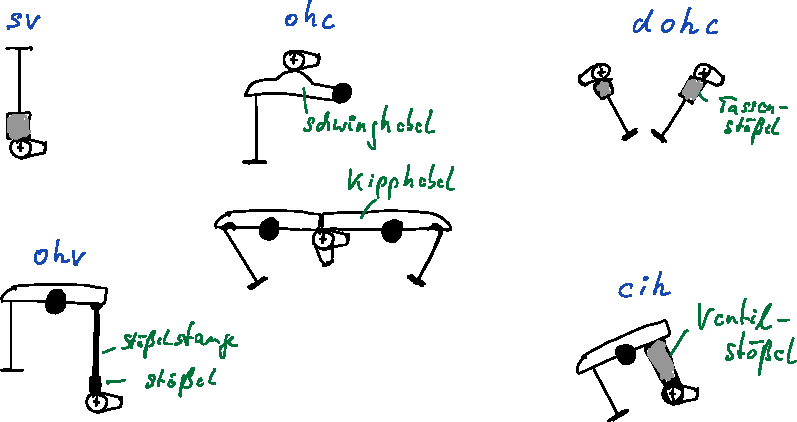
\includegraphics[width=0.6\textwidth]{images/Skizze/01_Anordnung-der-Nockenwelle_Skizze.pdf}
\caption{Anordnung der Nockenwelle}
%\label{fig:}%% anpassen
\end{figure}

\subsection{sv-Motor}\label{sv-motor}

\begin{itemize}
\item
  >>side valves<< seitlich stehende Ventile
\item
  untengesteuerter Motor
\item
  unten liegende Nockenwelle
\end{itemize}

\subsection{ohv-Motor}\label{ohv-motor}

\begin{itemize}
\item
  >>overhead valves<< hängende Ventile
\item
  obengesteuerter Motor
\item
  unten liegende Nockenwelle
\end{itemize}

\subsection{ohc-Motor}\label{ohc-motor}

\begin{itemize}
\item
  >>overhead camshaft<<
\item
  Nockenwelle über Zylinderkopf
\end{itemize}

\subsection{dohc-Motor}\label{dohc-motor}

\begin{itemize}
\item
  >>double overhead camshaft<<
\item
  zwei Nockenwellen über Zylinderkopf
\end{itemize}

\subsection{cih-Motor}\label{cih-motor}

\begin{itemize}
\item
  >>camshaft in head<<
\item
  Nockenwelle im Zylinderkopf
\end{itemize}

\section{Arten von
Nockenwellenantriebe}\label{arten-von-nockenwellenantriebe}

Fachbuch (\textcite{brand:2020:fachkundeKfz} S. 247)

\begin{enumerate}
\item
  Steuerkette
\item
  Zahnriemen
\item
  Königswelle
\item
  Stirnräder
\item
  Schubstangenmotoren
\end{enumerate}

\section{Nenne Zahnriemen Merkmale (trocken
laufend)}\label{nenne-zahnriemen-merkmale-trocken-laufend}

Fachbuch (\textcite{brand:2020:fachkundeKfz} S. 247)

\begin{itemize}
\item
  geringe Masse
\item
  geräuscharmer Lauf
\item
  begrenzte Standzeit, begrenzte Belastbarkeit
\item
  Unterliegen einem Wartungsintervall
\item
  braucht keine Schmierung
\item
  kostengünstig in der Produktion
\item
  Chemisch sensibel
\end{itemize}

\section{Ölbadzahnriemen Eigenschaften (nass
laufend)}\label{oelbadzahnriemen-eigenschaften-nass-laufend}

\begin{itemize}
\item
  mit Öl geschmierter Lauf
\item
  geringere Geräuschentwicklung
\item
  geringere Reibung ($20~\%$ weniger als Steuerkette)
\end{itemize}

\textbf{Ziel:}

\begin{itemize}
\item
  Kontaktflächen der beweglichen Teile reduzieren $\to$ Emissionen
\item
  Thermomanagement: Betriebstemperatur lange halten (BMW)
\end{itemize}

\section{Steuerkette Merkmale}\label{steuerkette-merkmale}

\begin{enumerate}
\item
  Große Kräfte übertragen
\item
  eigentlich wartungsarm, aus praktischer Sicht leider problembehaftet
\item
  teuer in Konstruktion
\item
  Steuerkette gilt als lauter
\item
  größere Masse als ein Riemen
\end{enumerate}

\section{Stirnradantrieb}\label{stirnradantrieb}

\begin{itemize}
\item
  Große Kräfte übertragen
\item
  wartungsfrei
\item
  schmale Bauform
\item
  teuer in Konstruktion
\item
  Dauerläufer (nicht problembehaftet)
\end{itemize}

\section{Königswelle}\label{koenigswelle}

\begin{itemize}
\item
  wartungsfrei
\item
  leicht, weil hohl gebohrt, Hohlröhre
\item
  kleine Kräfte übertragen
\item
  teuer in Konstruktion und Herstellung
\end{itemize}

\section{Unterschied - Steuern und
Regeln}\label{unterschied-steuern-und-regeln}

\subsection{Steuern}\label{steuern}

Soll-Ist-Vergleich

\begin{enumerate}
\def\labelenumi{\alph{enumi}.}
\setcounter{enumi}{25}
\item
  B. \emph{Steuerriemen}: Markierung soll auf OT stehen, alles in
  Ordnung, wenn nicht, dann defekt.
\end{enumerate}

\subsection{Regeln}\label{regeln}

Soll-Ist-Vergleich mit der Option des Eingriffs

\begin{enumerate}
\def\labelenumi{\alph{enumi}.}
\setcounter{enumi}{25}
\item
  B. \emph{ABS Regelkreis}: SG erfasst Drehzahlsignal, Drehen alle Räder
  gleich schnell, alles okay. Dreht ein Rad schneller $\to$ aktiver
  Eingriff ins System.
\end{enumerate}

\section{Nockenwellen -
Herstellungsmöglichkeiten}\label{nockenwellen-herstellungsmoeglichkeiten}

\subsection{Gegossene Nockenwelle}\label{gegossene-nockenwelle}

\begin{itemize}
\item
  muss nachgearbeitet werden, Lagerstellen, partiell gehärtet
\item
  biegsam, flexibles Bauteil (Gusseisen mit Lamellen- o. Kugelgrafit)
\item
  \emph{Vorteil} kostengünstig in der Herstellung, weniger
  problembehaftet
\end{itemize}

(\emph{Kaltverformen} je härter ein Material, um zu spröder.)

\subsection{Gebaute Nockenwelle}\label{gebaute-nockenwelle}

\begin{itemize}
\item
  zwei unterschiedliche Materialien,
\item
  Nocken (aus Einsatz-, Vergütungs- o. Nitrierstahl) auf ein Stahlrohr
  geschrumpft
\item
  \emph{Problem} Nocken können sich verdrehen
\item
  \emph{Vorteil} Gewichtsreduzierung, Nocken ist belastbarer
\item
  \emph{Nachteil} Aufwand
\item
  Material V4A (hohl gebohrt)
\end{itemize}

\section{Nockenformen}\label{nockenformen}

Fachbuch (\textcite{brand:2020:fachkundeKfz} S. 246)

\begin{figure}[!ht]% hier: !ht
\centering
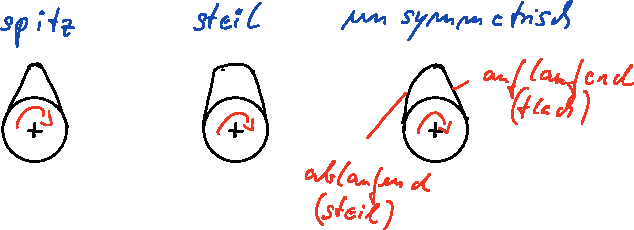
\includegraphics[width=0.6\textwidth]{images/Skizze/02_Nockenformen_Skizze.pdf}
\caption{Nockenformen}
%\label{fig:}%% anpassen
\end{figure}

\subsection{spitzer Nocken (tagenden
Nocken)}\label{spitzer-nocken-tagenden-nocken}

\begin{itemize}
\item
  langsames Öffnen / Schließen der Ventile
\item
  kurze Zeit voll geöffnet\\
\item
  geringe Füllung
\item
  stabiler Leerlauf
\item
  weicher und komfortorientierte Drehzahlbereich
\item
  nicht als hochdrehender, hochbelasteter Motor geeignet
\end{itemize}

\subsection{steiler Nocken (scharfer Nocken, Kreisbogen
Nocken)}\label{steiler-nocken-scharfer-nocken-kreisbogen-nocken}

\begin{itemize}
\item
  schnelles Öffnen / Schließen der Ventile
\item
  bleibt längere Zeit voll geöffnet
\item
  hoher Füllungsgrad, bei hohen Drehzahlen
\item
  im Leerlauf teilweise unrunder Lauf, da >>inneres AGR<< entstehen kann
  (große Ventilüberschneidung $\to$ Abgase in Ansaugtrakt) Abhilfe:
  Leerlaufdrehzahl erhöhen (750 $\to$ 950 U/min.)
\item
  Leistungsmotoren, hohe Drehzahlen
\end{itemize}

\subsection{unsymmetrischer Nocken}\label{unsymmetrischer-nocken}

\begin{itemize}
\item
  \emph{flach} langsameres öffnen der Ventile
\item
  \emph{steil} schnelles schließen der Ventile
\item
  längeres offen halten der Ventile
\item
  vereinigt beide Varianten
\end{itemize}

(\emph{Ziel bei hohen Drehzahlen}: Ventile schnell öffnen (Nocken) /
schließen (Ventilfeder) $\to$ gute Füllung, hohen Wirkungsgrad
erreichen.)

\section{Arten von
Ventilbetätigung}\label{arten-von-ventilbetaetigung}

Fachbuch (\textcite{brand:2020:fachkundeKfz} S. 247, 242)

\begin{figure}[!ht]% hier: !ht
\centering
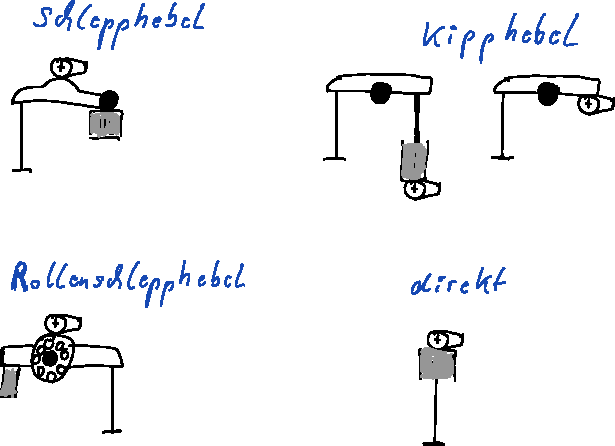
\includegraphics[width=0.6\textwidth]{images/Skizze/03_Arten-von-Ventilbetaetigung_Skizze.pdf}
\caption{Arten von Ventilbetätigung}
%\label{fig:}%% anpassen
\end{figure}

\subsection{Rollenschlepphebel, Schlepphebel,
Schwinghebel}\label{rollenschlepphebel-schlepphebel-schwinghebel}

\begin{itemize}
\item
  einarmige Hebel
\item
  geringe Reibung zwischen Nocken und Schlepphebel durch Nockenrolle
  (nadelgelagert)
\end{itemize}

\subsection{Kipphebel}\label{kipphebel}

zweiarmige Hebel

\subsection{direkt}\label{direkt}

Nockenwelle - Hydrostößel - Ventil

\section{Welche Beanspruchung ist das Ventil
ausgesetzt?}\label{welche-beanspruchung-ist-das-ventil-ausgesetzt}

\subsection{Mechanische Beanspruchung des
Ventils}\label{mechanische-beanspruchung-des-ventils}

\begin{itemize}
\item
  Ziehen (Ventilfeder, schließen, Ventilsitz)
\item
  Druck (Nocken, öffnen)
\item
  Torsion (verdrehen)
\item
  Biegen
\end{itemize}

\subsection{Chemische Beanspruchung}\label{chemische-beanspruchung}

Schwefel im Kraftstoff $\to$ Korrosion

\subsection{Thermische Belastung}\label{thermische-belastung}

Auslassventil bis $900^\circ\text{C}$

\section{Ventilspielausgleich}\label{ventilspielausgleich}

\textbf{Wofür?} Temperaturänderung (Motor Kaltstart, temperaturbedingte
Längenänderung des Ventils ausgleichen)

\textbf{Zu kleines Ventilspiel} (Nachteile)

\begin{itemize}
\item
  Ventil öffnet früher und schließt später
\item
  Ventil ist länger auf
\item
  kann dadurch nicht genügend Wärme abgeben über Ventilsitz
\item
  Ventilteller wird immer weiter einer höheren thermischen Belastung
  unterzogen und dadurch erhöhter Verschleiß
\item
  Am Ende ist das Ventil einer Hochtemperaturkorrosion unterworfen
  (Verbranntes Ventil)
\end{itemize}

\textbf{zu großes Ventilspiel} (Nachteile)

\begin{itemize}
\item
  Ventil öffnet zu spät, geht nicht ganz auf und schließt zu früh
\item
  Ventil ist kürzer auf
\item
  Klappergeräusche und erhöhter Verschleiß, \emph{Warum?} durch großes
  Ventilspiel, liegt nicht am Nockengrundkreis auf (Nocken schlägt auf
  Ventil)
\item
  Hieraus können folgen: schlechte Zylinderfüllung und die maximale
  erreichbare Leistung sinkt
\end{itemize}

\subsection{definiertes Ventilspiel}\label{definiertes-ventilspiel}

Wartung notwendig

\subsection{Hydraulischer
Ventilspielausgleich}\label{hydraulischer-ventilspielausgleich}

\textbf{ablaufender Nocken} (ohne Belastung)

\begin{itemize}
\item
  Entspannung des Systems
\item
  Spielausgleichsfeder drückt Druckbolzen nach oben bis Stößel am Nocken
  anliegt
\item
  Kugelventil öffnet sich, Raumvergrößerung im Arbeitsraum (Unterdruck)
\item
  Durch den Systemdruck strömt frisches Öl von außen ein und der
  Arbeitsraum wird befüllt
\end{itemize}

\textbf{auflaufender Nocken} (mit Belastung)

\begin{itemize}
\item
  Kugelventil schließt sich, es baut sich Druck im System auf
\item
  durch die Inkompressibilität von Flüssigkeiten $\to$ starre
  Verbindung
\item
  Nocken wird auf den Stößel auflaufen können, ohne Spiel zu haben und
  das Ventil betätigen
\item
  \emph{Warum Ringspalt?} (Wärmeausdehnung des Öls ausgleichen)
\item
  Wärmeeintrag: je wärmer das Öl, umso dünnflüssiger
\item
  dadurch wird >>Öl<< durch den kleinen Ringspalt gepresst (definierte
  Menge an Öl)
\item
  erfordert die richtige Öl-Viskosität (Zähflüssigkeit,
  Temperaturabhängig, Fließverhalten), sind an diese Ringspalte
  angepasst
\end{itemize}

Fachbuch (\textcite{brand:2020:fachkundeKfz} S. 245)

\begin{figure}[!ht]% hier: !ht
\centering
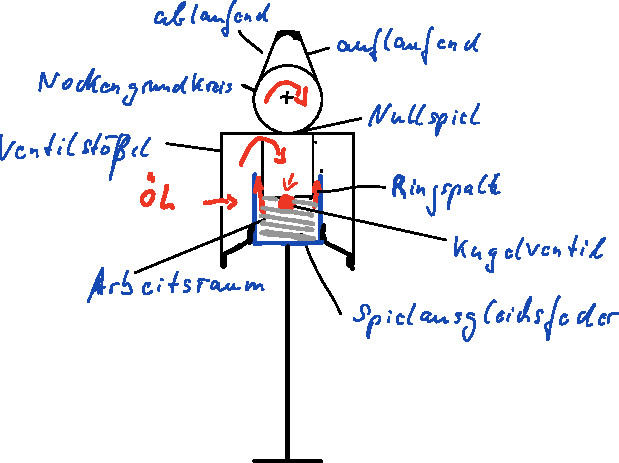
\includegraphics[width=0.6\textwidth]{images/Skizze/04_Ventilspielausgleich_Skizze.pdf}
\caption{Ventilspielausgleich}
%\label{fig:}%% anpassen
\end{figure}

\section{Drehzahlverhältnis zwischen Kurbelwelle zu
Nockenwelle?}\label{drehzahlverhaeltnis-zwischen-kurbelwelle-zu-nockenwelle}

2:1

\section{Was steuert die
Motorsteuerung?}\label{was-steuert-die-motorsteuerung}

Den Zeitpunkt und die Dauer des Ansaugens der Frischgase und den
Zeitpunkt und die Dauer des Ausstoßes der Abgase.

Öffnen und Schließen der Ventile.

\textbf{Voraussetzung}

\begin{enumerate}
\item
  Einspritzung des Kraftstoffs (Energieträger)
\item
  Eine Zündung, die diese Energie, gebunden im Kraftstoff, in chemische
  Energie, in Wärmeenergie umwandelt (Wärmekraftmaschine)
\end{enumerate}

Druck wird über eine Fläche in Kraft und Drehmoment übertragen, an die
Kurbelwelle übergeben, läuft durch das Getriebe - Achswellen - Reifen
auf die Straße und wir haben Vortrieb.

\section{Dreiventiltechnik mit zwei
Zündkerzen}\label{dreiventiltechnik-mit-zwei-zuendkerzen}

Fachbuch (\textcite{brand:2020:fachkundeKfz} S. 243)

Fachbuch (\textcite{respondeck:2019:servicetechniker} S. 142)

\subsection{Zusammenfassung}\label{zusammenfassung}

\begin{figure}[!ht]% hier: !ht
\centering
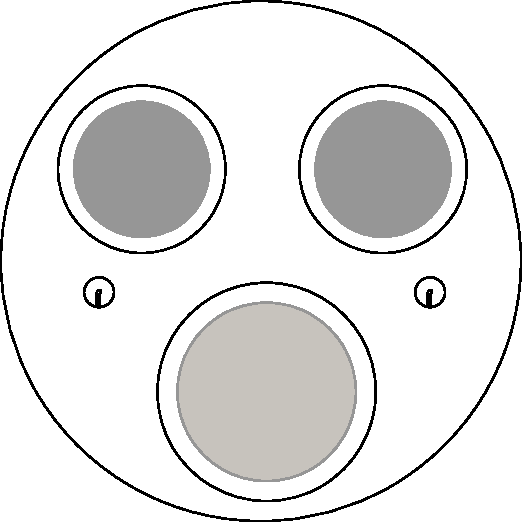
\includegraphics[width=0.2\textwidth]{images/Skizze/05_Dreiventiltechnik_Skizze.pdf}
\caption{Dreiventiltechnik}
%\label{fig:}%% anpassen
\end{figure}

Wir haben bei \textbf{drei Ventilen} einen großen Ein- und
Auslassquerschnitt.

Durch die Anordnung ist eine Unterbringung von \textbf{zwei Zündkerzen}
möglich, sodass zwei Zündkerzen in der Nähe der Zylinderwand entstehen
in deren Umgebung zwei Flammfronten. Somit kann bereits
niedergeschlagener Kraftstoff noch verdampfen und verbrannt werden.

Durch zwei Zündkerzen findet die Verbrennung schneller statt. Dadurch
wird der maximale Kolbendruck früher erreicht und ein hohes Drehmoment
erreicht. Wir nähern uns einer Gleichdruckverbrennung (Isobar).

\textbf{Klopfneigung} wird durch zwei Zündkerzen verringert. Da
geringere Wärmeeintrag in die noch nicht verbrannten Gase stattfindet.

\textbf{Abgastemperatur} ist niedriger, dadurch geringerer NOx-Ausstoß
trotz geringer HC und CO-Werte.

Dank nur \textbf{einem Abgasrohr} geringere Wärmeverluste. >>light off
point<< des Katalysators wird schneller erreicht.

\subsection{Warum sind das zwei Einlassventile und ein
Auslassventil?}\label{warum-sind-das-zwei-einlassventile-und-ein-auslassventil}

\textbf{Vorteil}

\begin{itemize}
\item
  kleine Massen
\item
  zwei kleine Ventile $\to$ große Einlassquerschnitte
\item
  höhere Drehzahlen
\item
  gute Füllung und Zylinderspülung
\end{itemize}

\textbf{Nachteil}

\begin{itemize}
\item
  mehr Teile $\to$ größere Reibungsverluste
\item
  Verschleiß und Ausfallwahrscheinlichkeiten
\end{itemize}

\textbf{Ein großes Ventil} hat eine Massenträgheit.

\begin{itemize}
\item
  Masse in Ruhelage (Ventil offen), Losbrechmoment~ $\to$ höchste
  Kraft, Masse in Bewegung (Federkraft: Ventil schließen)
\item
  Ansaugventil möglichst lange offen lassen (Kolben und Ventil kommen
  sich sehr nahe)
\item
  \emph{Ziel:} bestimmte Drehzahl erreichen (Wie schnell kann dieser
  Wechsel vollzogen werden?)
\end{itemize}

\subsection{Zylinderspülung bei
Ventilüberschneidung}\label{zylinderspuelung-bei-ventilueberschneidung}

Mit dem Ausstoß der Abgase ziehen wir einen kleinen definierten
Frischgasanteil mit, um den Zylinder zu spülen und möglichst wenig
inertes Gas (AGR) zu gewährleisten.

\subsection{Nachladeeffekt beim
Ansaugen}\label{nachladeeffekt-beim-ansaugen}

Einlassventile werden erst nach Durchschreiten des unteren Totpunktes
geschlossen. Frischgase strömen trotz aufwärtsgehendem Kolben in den
Zylinder nach. Die Kinetische Energie der einströmenden Frischgase ist
größer, als die Druckzunahme durch aufwärts gehenden Kolben.

\subsection{Warum zwei Zündkerzen?}\label{warum-zwei-zuendkerzen}

Zündkerze ist in der Nähe der Zylinderwand, zwei Flammenfronten
entstehen.

\begin{enumerate}
\item
  \textbf{Vollständige Verbrennung}

  \begin{itemize}
  \item
    niedergeschlagener Kraftstoff verdampft (an Zylinderwandung und
    Feuersteg) und der Verbrennung zugeführt
  \end{itemize}
\item
  \textbf{schnellerer Verbrennungsablauf}

  \begin{itemize}
  \item
    Schnelleres erreichen des maximalen Verbrennungsdruckes. Die
    Temperatur kann schneller konstant gehalten bzw. in Druck
    umgewandelt und über die Fläche des Kolbens in Kraft und Drehmoment
    auf die Kurbelwelle übertragen werden.
  \item
    Drehmoment = Kraft (max. Kolbendruck) x Hebelarm (90° stehende
    Kurbelwellenzapfen = Hebelarm am größten)
  \end{itemize}
\end{enumerate}

\subsection{Innermotorisch entstehen geringere
Schadstoffe}\label{innermotorisch-entstehen-geringere-schadstoffe}

\begin{enumerate}
\item
  \textbf{HC} geringer Ausstoß unverbrannter Kohlenwasserstoffe, durch
  weniger niedergeschlagener Kraftstoff
\item
  \textbf{CO} geringer, durch vollständige Verbrennung
\item
  \textbf{NOx} ist reduziert, durch schnelleren Verbrennungsablauf
  $\to$ zwei Zündkerzen, Abgastemperatur ist niedriger
\end{enumerate}

\subsection{Wann entsteht NOx?}\label{wann-entsteht-nox}

Durch hoher Druck und hohe Temperatur.

\subsection{Zusammenhang zwischen HC und CO
vs.~NOx}\label{zusammenhang-zwischen-hc-und-co-vs.-nox}

Es gibt zwei Zündgrenzen >>fett<< und >>mager<<.

\begin{enumerate}
\item
  \textbf{HC und CO} entsteht durch unvollständige fette Verbrennung

  \begin{itemize}
  \item
    Senken: durch Abmagern
  \item
    Verbrennungsspitzentemperatur: geringer
  \end{itemize}
\item
  \textbf{NOx} entsteht durch magere Verbrennung

  \begin{itemize}
  \item
    Senken: durch anfetten
  \item
    Verbrennungsspitzentemperatur: ansteigen
  \end{itemize}
\end{enumerate}

\subsection{Schadstoffe}\label{schadstoffe}

\begin{enumerate}
\item
  \textbf{HC} unverbrannte Kohlenwasserstoffe

  \begin{itemize}
  \item
    Verdampft am Ende der Verbrennung und wird dem Abgas zugeführt
  \end{itemize}
\item
  \textbf{CO} Kohlenmonoxid

  \begin{itemize}
  \item
    schwerer als Luft (Grube), bindet Hämoglobin im Blut
  \item
    keine vollständige Verbrennung
  \end{itemize}
\item
  \textbf{NOx} Stickoxide
\end{enumerate}

\subsection{Was ist AGR?}\label{was-ist-agr}

Platzhalter Gas (inertes Gas) nimmt nicht an der Verbrennung teil, soll
den Umgebungssauerstoff fernhalten

AGR-Rate ist am größten in Teillast (80 Km/h auf der Landstraße)

Ziel: Aus großen Motor $\to$ kleinen Motor machen, viel Abgas und
geringe Menge Kraftstoff einspritzen

\emph{Problem} >>Luftmenge ist da und kein Kraftstoff Einspritzen<<
$\to$ magere Verbrennung $\to$ thermische Belastung und Anstieg NOx

\emph{Luftmassenmesser} misst angesaugte Luftmasse und Sauerstoffgehalt
$\to$ AGR-Rate $\to$ Kraftstoffmenge berechnen

Ziel: homogen - Magerbetrieb (über den kompletten Zylinder)

\subsection{Wie entsteht Ruß?}\label{wie-entsteht-russ}

Kraftstoff wird an heißen Luft eingespritzt, zündfähiges
Kraftstoff-Luft-Gemisch bildet sich

\emph{einzelne Kraftstofftröpfchen}

\begin{itemize}
\item
  fangen von außen an zu verdunsten, entzünden, Verbrennung ist zu kurz
  (nicht vollständig)
\item
  innen: Verbrennung von Kohlenwasserstoff ohne Sauerstoff
\end{itemize}

\subsection{Was fördert die
Klopfneigung?}\label{was-foerdert-die-klopfneigung}

Unkontrollierte, unerwünschte Verbrennung (Glühzündung, klingende,
klopfende Verbrennung)

entzündet sich selbst an etwas glühenden, z. B. Ölkohle, Masseelektrode
(Zündkerze)

Wärme braucht Zeit zum Wirken.

\begin{enumerate}
\item
  \textbf{Wärmeeintrag gering:} geringe Klopfneigung, geringe thermische
  Belastung, schneller Verbrennungsablauf
\item
  \textbf{Wärmeeintrag hoch:} klopfende Verbrennung
\end{enumerate}

\subsection{Ein Auslassventil - ein
Abgasrohr}\label{ein-auslassventil-ein-abgasrohr}

Abgas verliert weniger Wärmeenergie.

\begin{enumerate}
\item
  ab ca. 450~°C >>light off point<< des Katalysators: min. $50~\%$ der
  Abgase konvertiert in nicht Schadstoffen
\item
  ab ca. 650 °C altert der Katalysator exponentiell und thermische
  Belastung
\end{enumerate}

\textbf{Thermodynamik - warme Luft strömt} schneller, weniger Rückstau.

Das unter Druck stehende Abgas verlässt den Zylinder mit Überschall
(Auspuffgeräusch). \textbf{Schallgeschwindigkeit} ca. 343 m/s (z. B.
Blitz $\to$ Donner, drei Sekunden zählen $\to$ ca. 1 km Entfernung)
 \newpage
\section{Lösung - Motorsteuerung}
%ju 08-Jun-22 02-Loesung-Motorsteuerung.tex
\textbf{1) Welche Aufgabe übernehmen die Ventile eines
Verbrennungsmotors?}

Ermöglicht den Gaswechsel und dichten den Verbrennungsraum gegenüber dem
Saugrohr und Abgasanlage ab.

\textbf{2) Warum haben Einlassventile meist einen größeren
Ventiltellerdurchmesser als Auslassventile?}

Einlassventile haben oftmals einen größeren Ventiltellerdurchmesser, da
das einströmende Frischgas nur durch Unterdruck im Zylinder angesaugt
wird, während das im Zylinder befindliche Altgas noch unter Restdruck
aus der Verbrennung steht und den Zylinder somit auch über einen kleinen
Querschnitt zuverlässig verlässt.

\textbf{3) Wie hoch ist die thermische Belastung von Ein- und
Auslassventilen?}

\textbf{Einlassventile} bis ca. $500^\circ\text{C}$
\textbf{Auslassventile} bis ca. $900^\circ\text{C}$ (fehlende
Frischgaskühlung)

\textbf{4) Welche Aufgabe hat die Ventildrehvorrichtung?}

Die Ventildrehvorrichtung hat die Aufgabe, die Ventile bei laufendem
Motor kontinuierlich zu drehen.

\textbf{Dies verhindert:}

\begin{enumerate}
\item
  ungleichmäßige Erwärmung der Ventilteller
\item
  Undichtigkeiten durch Verzug (nicht sauberes Anliegen)
\item
  Störungen bei Wärmeabgabe
\item
  Hochtemperaturkorrosion an den heißesten Stellen (das Ventil
  verbrennt)
\item
  Abblättern der Verbrennungsrückstände (stetiges Einschleifen der
  Ventile)
\end{enumerate}

\textbf{Bauformen}

\begin{enumerate}
\item
  Rotocap
\item
  Rotomat
\end{enumerate}

\textbf{5) Beschreiben Sie Aufbau und Wirkungsweise eines Hohlventils.
(inkl. Temperaturangaben!)}

Hohlventile sind im Schaft, teilweise auch im Teller hohl. Dieser
Hohlraum ist zu ca. $60 - 70~\%$ mit metallischem Natrium gefüllt, bei
ca. $98^\circ\text{C}$ schmilzt das Natrium und bewegt sich
hervorgerufen durch die Ventilbewegung im Ventil auf und ab. Bei jeder
Bewegung nimmt es am Ventilteller Wärme auf und gibt diese am
Ventilschaft ab. Der Abkühleffekt am Ventilteller liegt bei ca.
$80 - 150^\circ\text{C}$. Durch die hohlgeborte Form des Ventils
verringert sich seine Masse. Kann auch als Einlassventil verwendet
werden.

\textbf{6) Warum besteht zwischen dem Sitzwinkel des Ventilsitzringes im
Zylinderkopf und dem am Ventil oftmals eine Differenz von ca. 1°?}

Durch die Sitzwinkeldifferenz ist die Dichtfläche schmal. Bei
Inbetriebnahme des Motors arbeiten sich Ventilteller und Sitzring
schnell aufeinander ein. Dadurch entfällt das Ventileinschleifen.

(Flächenpressung, Minutenring)

\textbf{7) Welche Auswirkungen hat ein zu großes/zu kleines
Ventilspiel?}

\textbf{Zu kleines Ventilspiel} (Nachteile)

\begin{itemize}
\item
  Ventil öffnet früher und schließt später
\item
  Ventil ist länger auf
\item
  kann dadurch nicht genügend Wärme abgeben über Ventilsitz
\item
  Ventilteller wird immer weiter einer höheren thermischen Belastung
  unterzogen und dadurch erhöhter Verschleiß
\item
  Am Ende ist das Ventil einer Hochtemperaturkorrosion unterworfen
  (Verbranntes Ventil)
\end{itemize}

\textbf{zu großes Ventilspiel} (Nachteile)

\begin{itemize}
\item
  Ventil öffnet zu spät, geht nicht ganz auf und schließt zu früh
\item
  Ventil ist kürzer auf
\item
  Klappergeräusche und erhöhter Verschleiß, \emph{Warum?} durch großes
  Ventilspiel, liegt nicht am Nockengrundkreis auf (Nocken schlägt auf
  Ventil)
\item
  Hieraus können folgen: schlechte Zylinderfüllung und die maximale
  erreichbare Leistung sinkt
\end{itemize}

\textbf{8) Wo im Ventiltrieb kann der Ventilspielausgleich eingesetzt
sein?}

Ventilspielausgleich kann sich zwischen Nocken und Ventil oder bei
Bauformen Schlepphebel am Aufnahmepunkt des Hebels befinden.

\textbf{9) Beschreiben Sie Aufbau und Wirkungsweise des hydraulischen
Stößel.}

\textbf{Ablaufender Nocken} (ohne Belastung)

\begin{itemize}
\item
  Entspannung des Systems
\item
  Spielausgleichsfeder drückt Druckbolzen nach oben bis Stößel am Nocken
  anliegt
\item
  Kugelventil öffnet sich, Raumvergrößerung im Arbeitsraum (Unterdruck)
\item
  Durch den Systemdruck strömt frisches Öl von außen ein und der
  Arbeitsraum wird befüllt
\end{itemize}

\textbf{Auflaufender Nocken} (mit Belastung)

\begin{itemize}
\item
  Kugelventil schließt sich, es baut sich Druck im System auf
\item
  durch die Inkompressibilität von Flüssigkeiten $\to$ starre
  Verbindung
\item
  Nocken wird auf den Stößel auflaufen können, ohne Spiel zu haben und
  das Ventil betätigen
\item
  \emph{Warum Ringspalt?} (Wärmeausdehnung des Öls ausgleichen)
\item
  Wärmeeintrag: je wärmer das Öl, umso dünnflüssiger
\item
  dadurch wird >>Öl<< durch den kleinen Ringspalt gepresst (definierte
  Menge an Öl)
\item
  erfordert die richtige Öl-Viskosität (Zähflüssigkeit,
  Temperaturabhängig, Fließverhalten), sind an diese Ringspalte
  angepasst
\end{itemize}

\textbf{10) Warum verwendet man bei herkömmlichen 4-Takt-Motoren und
Pkw-Dieselmotoren nur noch oben liegende Nockenwellen?}

Durch die obenliegende Nockenwelle können die bewegten Massen des
Ventiltriebs gering gehalten und somit höhere Drehzahlen erreicht
werden. (z. B. Stößelstange, mehr Bewegung $\to$ erhöht Reibung und
Masse)

\textbf{11) Welche Nockenausführungen findet man an den Nockenwellen von
Verbrennungsmotoren?}

\begin{enumerate}
\item
  \textbf{spitzer Nocken} (tagenden Nocken)
\item
  \textbf{steiler Nocken} (scharfer Nocken, Kreisbogen Nocken)
\item
  \textbf{unsymmetrischer Nocken}
\end{enumerate}

\textbf{12) Aus welchem Werkstoff können Nockenwellen bestehen? (keine
Prüfung)}

\begin{enumerate}
\item
  \textbf{Gegossene Nockenwelle}

  \begin{itemize}
  \item
    Gusseisen mit Lamellen- o. Kugelgrafit
  \end{itemize}
\item
  \textbf{Gebaute Nockenwelle}

  \begin{itemize}
  \item
    Einsatz-, Vergütungs- o. Nitrierstahl
  \end{itemize}
\end{enumerate}

(Eigenschaften: Welche Kräfte wirken? zäh fest versus beweglich)

\textbf{13) Was versteht man unter desmodromischer Ventilsteuerung?}

Bei desmodromischer Ventilsteuerung werden die Einlassventile und
Auslassventile jeweils durch einen Öffnungs- und Schließkipphebel
betätigt.

(Zwangssteuerung, Einsatz: hohe Drehzahlen, AV zuverlässig schließen)

\chapter{Füllungsoptimierung I}
%ju 05-Jun-22 03-Fuellungsoptimierung-I.tex
\section{Downsizing (Prüfung)}\label{downsizing-pruefung}

Verkleinerung der Motoren (Hubraum und Zylinderzahl) bei gleicher
Leistung.

\section{LSPI - Low
Speed-Pre-Ignition}\label{lspi-low-speed-pre-ignition}

LSPI = vorzeitige Zündung, betrifft hoch aufgeladene Downsizing Motoren
\footnote{\url{https://www.autobild.de/artikel/lspi-vorzeitige-zuendung-16385077.html}}

\begin{itemize}
\item
  \textbf{Turbo aufgeladene Motoren}

  \begin{itemize}
  \item
    geringes Verdichtungsverhältnis (7-8:1)
  \item
    vor verdichtete Luft wird in den Zylinder eingeblasen und verdichtet
  \item
    Ladedruckregelung (Lastwunsch)
  \item
    vorgewärmte Luft (Ladeluftkühlung)
  \end{itemize}
\item
  vs.~\textbf{hoch verdichtete Saugmotoren}

  \begin{itemize}
  \item
    hohes Verdichtungsverhältnis (10-11:1), endet bei Klopfgrenze
  \end{itemize}
\end{itemize}

\textbf{Zwei Zündquellen, Ursache für die Selbstentzündung}

\begin{enumerate}
\item
  Niedergeschlagen Kraftstoff in Verbindung mit sehr niedrig Viskoses Öl

  \begin{itemize}
  \item
    $\to$ ein brennbares Gemisch entsteht, mit einer nicht ganz
    bekannten Selbstentzündungstemperatur
  \end{itemize}
\item
  Ölkohlerückstände (Kraftstoffreste) im Bereich der Einspritzdüsen
\end{enumerate}

Durch eine überhohe Verdichtung $\to$ steigt Verdichtungsenddruck und
damit Verdichtungstemperatur $\to$ dadurch hohe thermische Belastung.
Die Folge ist ein kapitaler Motorschaden.

\textbf{Körnerschlag} \footnote{\url{https://cdn.germanscooterforum.de/monthly_05_2009/post-24449-1241606436.jpg}}
Kolbenschäden $\to$ es entsteht eine Druckspritze bevor der Kolben OT
erreicht, eine zweite Flammenfront entsteht, wenn jetzt zwei
Flammfronten aufeinandertreffen, entstehen sehr hohe Druckspitzen, auch
wenn der Kolben nach UT geht.

\textbf{Kavitation} \footnote{\url{https://prozesstechnik.industrie.de/wp-content/uploads/4/0/40278086.jpg}}
Dampfblasenbildung \footnote{\url{https://www.youtube.com/watch?v=SEGTFbZ5RJ8}}
z. B. Bootsschraube saugt Flüssigkeiten an, Druck fällt ab durch
Unterdruck, wenn jetzt die Gasblasen implodieren, entstehen sog.
Mikrojets $\to$ Druckspitzen.

\section{Vorteile von Downsizing
Motoren}\label{vorteile-von-downsizing-motoren}

\begin{enumerate}
\item
  Geringere Pumpverluste (2 l vs.~1,2 l bei gleicher Leistung 150 PS)
\item
  geringere Reibungsverluste aufgrund der geringeren Größe
\item
  weniger Wärmeübertrag von Gasen zur Zylinderwandung
\end{enumerate}

\section{Mehrventiltechnik}\label{mehrventiltechnik}

Fachbuch (\textcite{respondeck:2019:servicetechniker} S. 141)

Um die Zylinderfüllung zu verbessern, werden drei oder mehr Ventile pro
Zylinder in Verbrennungsmotoren eingesetzt.

\textbf{Ziele von Mehrventiltechnik}

\begin{itemize}
\item
  Öffnungsquerschnitt der Ventile vergrößern, ohne die
  Drehzahlfestigkeit durch größere und damit trägere Ventile (mehr
  Masse) zu mindern.
\end{itemize}

\textbf{Vor- und Nachteile von Mehrventiltechnik}

\begin{itemize}
\item
  bessere Zylinderfüllung
\item
  Drehzahlfest
\item
  innere Reibung steigt
\item
  Abgaswärmeentzug

  \begin{itemize}
  \item
    Der Katalysator kommt schlechter auf Betriebstemperatur, da sich die
    Abgase an den Abgasrohren abkühlen können.
  \item
    Je mehr Auslassventile vorhanden sind, desto größer ist die
    Oberfläche der Abgasrohre und desto mehr kühlen die Abgase aus.
  \end{itemize}
\end{itemize}

Honda NR 750 - Ovalkolben \footnote{\url{https://de.wikipedia.org/wiki/Honda_NR_750}}

\textbf{Dreiventiltechnik} (Vorteile)

\begin{itemize}
\item
  Verbrennungsdruck steigt (kürzere Flammwege)
\item
  geringere Klopfneigung (weniger Zeit zur Gemischerwärmung vor
  Verbrennungsbeginn)
\item
  Ausstoß unverbrannter Kohlenwasserstoffe verringert sich (Zündkerze
  ist in der Nähe der Zylinderwand, wo das Kondensat lagert)
\item
  geringere NOx
\end{itemize}

Vgl. Kapitel >>\emph{Motorsteuerung / Dreiventiltechnik mit zwei
Zündkerzen}<<

\section{Nockenwellenverstellung - variable
Steuerzeiten}\label{nockenwellenverstellung-variable-steuerzeiten}

Fachbuch (\textcite{brand:2020:fachkundeKfz} S. 249)

Verdrehen der Einlassnockenwelle bzw. der Ein- und Auslassnockenwelle,
abhängig von der Motordrehzahl, Motorlast und Temperatur. Hierdurch
lässt sich die \emph{Länge der Ventilüberschneidung} anpassen.

\textbf{Warum machen wir eine Nockenwellenverstellung?} (Vorteile)

\begin{enumerate}
\item
  Optimale Zylinderfüllung in den unterschiedlichen Last- und
  Drehzahlbereichen zu ermöglichen
\item
  inneres AGR
\end{enumerate}

\textbf{Ziele der Nockenwellenverstellung}

\begin{itemize}
\item
  Wann das Ventil öffnet und schließt zu beeinflussen (variabel)
\item
  bei gleichbleibenden Nocken, Dauer und Öffnungswinkel (Hub) ändern
  sich nicht
\item
  Verdrehrichtung der Nockenwelle: Früh, Spät
\end{itemize}

\textbf{Verstellung der Einlassnockenwelle in Abhängigkeit vom
Betriebszustand}

\begin{table}[!ht]% hier: !ht 
\centering 
	\caption{}% \label{tab:}%% anpassen 
\begin{tabular}{@{}llll@{}}
\hline
\textbf{Betriebszustand} & \textbf{Leerlauf} & \textbf{Teillast} &
\textbf{Volllast} \\
\hline
Verstellrichtung NW & Spät & Früh & Spät \\
Ventilüberschneidung & klein & groß & klein \\
Abgas & CO sinkt & NOx sinkt & \\
EV schließt & weit nach UT & kurz nach UT & weit nach UT \\
\hline
\end{tabular} 
\end{table}

Merkmale (Vgl. Tabelle Verstellung der Einlassnockenwelle in
Abhängigkeit vom Betriebszustand)

\begin{itemize}
\item
  \textbf{Leerlauf} Kein Überströmen von Frischgasen und Abgasen,
  besserer Verbrennungsverlauf
\item
  \textbf{Teillast} Abgase strömen in den Einlasskanal und werden mit
  den Frischgasen angesaugt. Temperatur sinkt, NOx-Anteil sinkt
\item
  \textbf{Volllast} \emph{Nachladeeffekt} Frischgase strömen trotz
  aufwärts gehenden Kolben in den Zylinder nach
\end{itemize}

\textbf{Ausgangspunkt} $\to$ 90er-Jahre, erste Form des AGR (inneres
AGR), Drei-Wege-Katalysator, Ottomotor, Euro 2, Teillast (höchste
AGR-Rate, 80 km/h auf der Landstraße, keine Lastabfrage,
Spritspareffekt, NOx-Anteil senken)

\subsection{VarioCam - Verstellbarer Kettenspanner (Audi,
VW)}\label{variocam-verstellbarer-kettenspanner-audi-vw}

$\to$ Verändern der Ventilöffnungszeit der Einlassnockenwelle

\textbf{Wie?} Vgl. Tabelle Verstellung der Einlassnockenwelle in
Abhängigkeit vom Betriebszustand

\begin{itemize}
\item
  KW treibt Auslass-NW an und diese über einer Kette die Einlass-NW
\item
  \textbf{Kettenspanner} spannt \textbf{Kette nach oben} (federbelastet)
\item
  \textbf{NW} dreht sich \textbf{gegen UZS} (Uhrzeigersinn) in
  \textbf{Verstellposition} >>spät<< (Ausgangslage, Ventilüberschneidung
  klein)
\item
  SG bestromt Magnetventil, Motoröl fließt in Kettenspanner.
\item
  \textbf{Kettenspanner} spannt \textbf{Kette nach unten}
  (Hydraulikzylinder)
\item
  \textbf{NW} dreht sich \textbf{im UZS} in \textbf{Verstellposition}
  >>früh<<, (Ventilüberschneidung groß)
\end{itemize}

\subsection{Vanos - Variable Nockenwellensteuerung
(BMW)}\label{vanos-variable-nockenwellensteuerung-bmw}

\textbf{Wie?}

\begin{itemize}
\item
  \textbf{Nockenwellenrad und Nockenwelle} sind über ein \textbf{steiles
  Gewinde} miteinander verbunden.
\item
  \emph{Grundposition} NW steht in \textbf{Verstellposition} >>spät<<
\item
  SG bestromt ein Magnetventil (4/2-Wegeventil) $\to$ gibt den
  \textbf{Ölzufluss} zum Frühkanal frei
\item
  NW verdreht sich gegen Uhrzeigersinn in \textbf{Verstellposition}
  >>früh<<
\item
  Durch wechselseitigen Druckaufbau lässt sich die Position der
  Verstelleinheit halten.
\end{itemize}

\subsection{Flügelzellenversteller
(Mercedes)}\label{fluegelzellenversteller-mercedes}

$\to$ Verändern der Steuerzeiten

\textbf{Wie?}

\begin{itemize}
\item
  \textbf{Innenrotor} (fest mit NW) \textbf{und Außenrotor} (fest mit
  Kettenrad)
\item
  SG bestromt \textbf{Magnetventil} $\to$ die \textbf{Ölräume}
  zwischen den Rotorblättern können wechselseitig mit Öl befüllt werden
\item
  Die Kraftübertragung vom Nockenwellenrad auf die NW erfolgt immer über
  das Öl.
\item
  wird Ölraum rechts vom Innenrotorblatt mit Öl befüllt, kommt es zu
  einer \textbf{Verdrehung der NW gegen UZS} (Uhrzeigersinn) in Richtung
  >>spät<<
\item
  wird Ölraum links vom Innenrotorblatt mit Öl befüllt, kommt es zu
  einer \textbf{Verdrehung der NW im UZS} in Richtung >>früh<<
\item
  Durch wechselseitigen Druckaufbau lässt sich die Position der
  Verstelleinheit halten.
\end{itemize}

\section{Variabler Ventiltrieb}\label{variabler-ventiltrieb}

\subsection{Stufenweise variabler
Ventiltrieb}\label{stufenweise-variabler-ventiltrieb}

\textbf{Vorteile}

Bessere Zylinderfüllung durch zwei unterschiedliche Nockenprofile

\begin{itemize}
\item
  \emph{obere Drehzahlbereich} $\to$ steiler Nocken

  \begin{itemize}
  \item
    schnelles Öffnen, lange Öffnungsdauer, schnelles Schließen
  \end{itemize}
\item
  \emph{untere Drehzahlbereich} $\to$ spitzer Nocken

  \begin{itemize}
  \item
    Verhinderung von ungewollter Abgasrückführung durch zu lange
    Ventilüberschneidung
  \end{itemize}
\end{itemize}

\subsubsection{VTEC - Variable Valve Timing and Lift Electronic Control
(Honda)}\label{vtec-variable-valve-timing-and-lift-electronic-control-honda}

$\to$ Verändern von Ventilhub und Ventilöffnungszeit

\textbf{Wie?}

\begin{itemize}
\item
  Verstelleinheit liegt in den Schlepphebeln
\item
  \textbf{Umschaltung} zwischen dem Nockenprofilen erfolgt durch
  \textbf{Verblocken der Schlepphebel}
\item
  \textbf{Schlepphebel entriegelt}

  \begin{itemize}
  \item
    Die beiden äußeren Nocken öffnen mithilfe der äußeren Schlepphebel
    die Ventile.
  \item
    \textbf{Spitzer Nocken}

    \begin{itemize}
    \item
      kleiner Ventilhub
    \item
      kurze Ventilöffnungszeit
    \item
      \emph{niedrige Drehzahlen}
    \end{itemize}
  \end{itemize}
\item
  SG bestromt Elektromagnet, \textbf{Öldruck} verschiebt die
  \textbf{Sperrschieber} und verblockt die Schlepphebel untereinander.
\item
  \textbf{Schlepphebel verriegelt}

  \begin{itemize}
  \item
    wenn der steile Nocken auf den mittleren Schlepphebel aufläuft,
    nimmt dieser die beiden äußeren Schlepphebel mit und diese öffnen
    die Ventile.
  \item
    \textbf{Steiler Nocken}

    \begin{itemize}
    \item
      großer Ventilhub
    \item
      lange Ventilöffnungszeit
    \item
      \emph{hohe Drehzahlen}
    \end{itemize}
  \end{itemize}
\end{itemize}

\subsubsection{VarioCam Plus (Porsche)}\label{variocam-plus-porsche}

$\to$ Verändern von Ventilhub und Ventilöffnungswinkel

\textbf{Wie?}

\begin{itemize}
\item
  Verstelleinheit liegt im Tassenstößel
\item
  SG bestromt \textbf{Elektromagnet}, damit wird der
  \textbf{Tassenstößel mit Öldruck} gesteuert
\item
  Diese bestehen aus \textbf{zwei Stößeln}, die mithilfe eines
  \textbf{Bolzens} gegeneinander verriegelt werden können.
\item
  innere Stößel $\to$ kleinen Nocken
\item
  äußere Stößel $\to$ großen Nocken
\item
  \textbf{Stößel verriegelt} $\to$ große Ventilhub

  \begin{itemize}
  \item
    Innere und äußere Stößel wird durch einen Bolzen verriegelt
  \end{itemize}
\item
  \textbf{Stößel entriegelt} $\to$ kleiner Ventilhub

  \begin{itemize}
  \item
    sinkt der Öldruck, wird durch die Federkraft der Bolzen
    zurückgeschoben
  \end{itemize}
\end{itemize}

\subsubsection{Valvelift (Audi, +
Zylinderabschaltung)}\label{valvelift-audi-zylinderabschaltung}

\textbf{Wie?}

\begin{itemize}
\item
  Änderung des Nockenprofils durch Verschieben der Verstelleinheit
  (Nockenstück) auf der NW
\item
  SG bestromt \textbf{Elektromagnet} $\to$ \textbf{Metallstift} fährt
  aus \textbf{in eine Spiralnut} und verschiebt das \textbf{Nockenstück}
\item
  damit schalte ich zwischen \textbf{zwei Nockenprofilen} um
\item
  Arretierung des Nockenstücks erfolgt durch eine federbelastete Kugel.
\item
  \textbf{Zylinderabschaltung} (Teillast)

  \begin{itemize}
  \item
    Nockenprofil $\to$ Nockengrundkreis
  \item
    Die Ventile bleiben bei abgeschaltetem Zylinder geschlossen.
  \end{itemize}
\end{itemize}

\subsection{Stufenlos variabler
Ventiltrieb}\label{stufenlos-variabler-ventiltrieb}

\textbf{Vorteile}

$\to$ Verändern von Ventilhub in allen Drehzahlbereichen

\textbf{Ziel im unteren Drehzahlbereich}: Ein zündbares Gemisch zu
realisieren.

\textbf{Wie?}

\begin{itemize}
\item
  Durch geringe Ventilöffnung und damit Erhöhung der
  Strömungsgeschwindigkeit der Frischgase

  \begin{itemize}
  \item
    >>Venturi-Prinzip<< eine Verengung in einem Strömungskanal

    \begin{itemize}
    \item
      $\to$ höhere Strömungsgeschwindigkeit
    \item
      $\to$ bessere Verwirbelung
    \item
      $\to$ bessere Verteilung des Kraftstoff-Luftgemisches
    \end{itemize}
  \end{itemize}
\item
  Drosselklappe könnte wegfallen, wird aber weiterhin verbaut
\item
  \textbf{Wozu ist die Drosselklappe dann noch notwendig?}

  \begin{itemize}
  \item
    Schaltung des AGR (Abgasrückführung)

    \begin{itemize}
    \item
      Aufbau eines Druckgefälles/Druckdifferenz, durch Schließen der
      Drosselklappe wird ein Unterdruck erzeugt, was dazu führt, dass
      die Abgase in den Ansaugtrakt einströmen können
    \end{itemize}
  \end{itemize}
\item
  Notlauf
\end{itemize}

\subsubsection{Valvetronic}\label{valvetronic}

$\to$ Verändern von Ventilöffnungswinkel (Hub) und Ventilöffnungsdauer
(Nockenwellenverstellung)

\textbf{Wie?}

\begin{itemize}
\item
  SG verdreht mithilfe eines \textbf{Stellmotors} eine
  \textbf{Exzenterwelle} (Halbmondförmig)
\item
  Druck des Nockens wird zunächst auf einen \textbf{Zwischenhebel}
  übertragen
\item
  Der \textbf{Leerweg}, den der Zwischenhebel von der Betätigung durch
  den Nocken bis zur Übertragung auf das Ventil durchläuft, ist mittels
  einer Exzenterwelle einstellbar.
\item
  Je größer der Leerweg, desto kleiner der Ventilhub.
\item
  \textbf{Ventilhub} 0,3 mm und 9,85 mm
\end{itemize}

\subsubsection{Elektrohydraulischer Ventiltrieb
(MultiAir)}\label{elektrohydraulischer-ventiltrieb-multiair}

\textbf{Vorteil} Vollvariable Steuerzeiten

$\to$ stufenlose Veränderung von Ventilhub, Ventilöffnungsdauer und
die Anzahl der Ventilhübe der EV

\textbf{Wie?}

\begin{itemize}
\item
  auf der \textbf{Auslassnockenwelle} gibt es einen
  \textbf{Extranocken}, über Schlepphebel wird ein
  \textbf{Pumpenelement} betätigt

  \begin{itemize}
  \item
    $\to$ der erzeugt einen \textbf{Öldruck}, um die
    \textbf{Einlassseite} zu steuern,
  \end{itemize}
\item
  \textbf{Magnetventil geschlossen} Druck wird auf den Kolben
  übertragen, Ventil öffnen
\item
  \textbf{Magnetventil offen} Ventil schließen. Der Öldruck fließt in
  den Druckspeicher ab.
\item
  \emph{Vorteil \textbf{Druckspeicher}:} von der Nockenwelle
  unabhängiger Zeitpunkt, mit Öffnung eines Magnetventils (SG) ein
  Öldruck aus dem Druckspeicher nutzen, der das \textbf{Ventil
  öffnet/schließt}
\item
  \textbf{elektrohydraulisch-pneumatisch} (Ventile unabhängig von NW
  betätigen, noch nicht in der Großserie)
\item
  chinesische Hersteller Qoros und der schwedische
  Luxussportwagenhersteller Königsegg
\end{itemize}

\subsubsection{Elektromagnetischer Ventiltrieb (noch nicht zur
Serienreife
geschafft)}\label{elektromagnetischer-ventiltrieb-noch-nicht-zur-serienreife-geschafft}

\textbf{Vorteile}

\begin{itemize}
\item
  Vollvariable Steuerzeiten
\item
  Anzahl der geöffneten Ventile pro Zylinder frei wählbar
\item
  Zylinderabschaltung (ohne Gaswechselverluste möglich)
\item
  Wegfall von Nockenwellen (Gewichtseinsparung)
\end{itemize}

\textbf{Wie?}

\begin{itemize}
\item
  Unterstützung des Elektromagneten beim schnellen Öffnen und Schließen
  des Ventils.
\item
  Abbremsen des Ventils kurz vor den Endstellungen geöffnet und
  geschlossen
\item
  Ventile beim abgeschalteten oder defekten Systems in halbgeöffnete
  Stellung bringen, um Motorschäden durch Aufsetzen der Ventile zu
  verhindern.
\end{itemize}
 \newpage
\section{Lösung - Füllungsoptimierung I}
%ju 11-Jun-22 03-Loesung-Fuellungsoptimierung-I.tex
\textbf{1) Warum werden die herkömmlichen Serienmotoren statt mit 2
häufig mit 3 oder 4 Ventilen ausgerüstet?}

Mehrventiltechnik ermöglicht eine \textbf{bessere Zylinderfüllung} durch
\textbf{Vergrößerung des Ein- und Auslassquerschnittes} und
\textbf{Verbesserung der Strömungsverhältnisse} im Zylinder. Dies wäre
bedingt auch durch größere Ein- und Auslassventile möglich. Würde aber
aufgrund der \textbf{größeren bewegten Massen} im Ventiltrieb die
\textbf{Drehzahlfestigkeit} herabsetzen.

\textbf{2) Warum rüstet man einen Dreiventilmotor mit 2 Zündkerzen und
Doppelzündung aus?}

\begin{enumerate}
\item
  Kontrollierte schneller Druckanstieg
\item
  Kondensierte Kraftstoffbestandteile an der Zylinderwand können durch
  den Verbrennungsbeginn in Zylinderwandnähe wieder vergasen und wieder
  an der Verbrennung teilnehmen.

  \begin{itemize}
  \item
    Geringere $\text{HC}$-Ausstoß
  \end{itemize}
\item
  Geringe Aufheizung des Gemisches vor der Verbrennung

  \begin{itemize}
  \item
    Geringe Klopfneigung und geringe $\text{NO}_\text{x}$-Ausstoß
  \end{itemize}
\end{enumerate}

\textbf{3) Was versteht man unter variabler Ventilsteuerung?}

Bei der variablen Ventilsteuerung werden die \textbf{Steuerzeiten} der
Einlass- und in manchen Fällen auch die der AV bedarfsgerecht \textbf{in
Abhängigkeit von Drehzahl und Last} verändert. Dies geschieht
\textbf{durch Verdrehen der Einlass- bzw. Auslass-NW}.

\textbf{4) Beschreiben Sie Aufbau und Funktion der >>Vario-Cam<< -
Nockenwellenverstellung.}

Das Vario-Cam System besteht aus einer direkt von der KW des Motors
angetriebenen Auslass-NW und einer von der Auslass-NW angetrieben
Einlass-NW.

Der \textbf{Kettenspanner} der zwischen den NW liegenden Steuerkette ist
in der Lage diese sowohl nach oben als auch nach unten zu spannen.

Spannt er die \textbf{Kette nach oben,} wird die \textbf{Einlass-NW
gegen den UZS} (Uhrzeigersinn) in die \textbf{Verstellposition spät}
gebracht.

Spannt der Kettenspanner die \textbf{Kette nach unten,} so verdreht die
\textbf{Einlass-NW im UZS} (Uhrzeigersinn) in \textbf{Verstellposition
früh}.

\textbf{5) Welchen Vorteil bietet das VTEC-System gegenüber einem
herkömmlichen Ventiltrieb?}

Beim VTEC-System kommen im unteren Drehzahlbereich \textbf{spitze} und
im oberen Drehzahlbereich \textbf{steilen Nocken} zum Einsatz.

Hierdurch wird gewährleistet, dass der Gaswechsel im Zylinder im
\textbf{unteren Drehzahlbereich} (viel Zeit) stattfinden kann,
\textbf{ohne die Beimischung von Altgas} durch zu frühes Öffnen der
Einlassventile zu riskieren.

Jedoch auch im \textbf{oberen Drehzahlbereich} (wenig Zeit) mithilfe
einer geänderten Nockenprofils mit längeren Ventilöffnungszeiten ein
\textbf{zuverlässiger Gaswechsel} gewährleistet werden kann.

\textbf{6) Wodurch erfolgt die Umschaltung zwischen den Nockenprofilen
beim Valvelift-System?}

Beim Valvelift-System wird, sobald das SG dies veranlasst, ein
\textbf{Elektromagnet bestromt,} wodurch ein \textbf{Metallstift}
ausfährt, der bei ablaufenden Nocken in eine dafür vorgesehene
\textbf{Verstellnut} einfährt und die gesamte Verstelleinheit auf der
Nockenwelle um ca. $7~mm$ verschiebt bis der \textbf{zweite Nocken}
gerade über den Rollenschlepphebel steht.

\textbf{7) Welche Aufgabe haben die Kompressions- und
Dekompressionsfedern eines elektromagnetischen Ventiltriebs?}

\begin{itemize}
\item
  \textbf{Unterstützung} des Elektromagneten \textbf{beim schnellen
  Öffnen und Schließen} des Ventils.
\item
  \textbf{Abbremsen des Ventils} kurz vor den Endstellungen geöffnet und
  geschlossen
\item
  Ventile beim abgeschalteten oder defekten Systems \textbf{in
  halbgeöffnete Stellung} bringen, um Motorschäden durch Aufsetzen der
  Ventile zu verhindern.
\end{itemize}

\chapter{Füllungsoptimierung II}
%ju 28-Jun-22 04-Fuellungsoptimierung-II.tex
\section{Wie beschreiben Sie die Dynamische
Aufladung?}\label{wie-beschreiben-sie-die-dynamische-aufladung}

\textbf{Ausgangslage} Ansaugen, Volumenvergrößerung, Druckdifferenz

Die \textbf{einströmenden Frischgase} werden am geschlossenen Ventil
\textbf{reflektiert} und an der bereits im Ansaugrohr stehenden
Luftmasse (Außenluft) erneut reflektiert und bewegt sich wieder auf das
EV zu und wenn jetzt das Ventil öffnet können die Frischgase schneller
in den Zylinder einströmen, weil die \textbf{Massenträgheit} einer
ruhenden Luftmasse nicht überwunden werden muss.

Wir machen uns hier die \textbf{kinetische Energie} der sich bereits
\textbf{in Bewegung gesetzten Luftmasse} zunutze, sodass der Beginn des
Einströmens kein Losbrechmoment der Luftmasse darstellt, sondern eine
schon in sich bewegten Luftmasse/Luftsäule zu nutzen und lässt damit das
\textbf{Einströmen schneller beginnen} und dadurch wird ein besserer
Füllungsgrad erreicht (Frischgasanteil steigt, mehr Kraftstoff $\to$
mehr Leistung und Drehmoment).

\subsection{Schwingsaugrohr}\label{schwingsaugrohr}

Variante

\begin{enumerate}
\item
  \textbf{Schaltsaugrohr} einfaches umschalten zwischen

  \begin{itemize}
  \item
    \textbf{lange Saugrohrlänge} und großes Sammlervolumen, große Massen
    (sind träge)

    \begin{itemize}
    \item
      \textbf{unteren Drehzahlbereich}
    \item
      Klappe geschlossen
    \end{itemize}
  \item
    \textbf{kurze Saugrohrlänge}, kleine Massen (sind agiler)

    \begin{itemize}
    \item
      \textbf{oberen Drehzahlbereich}
    \item
      Klappe offen
    \item
      Gassäule kann direkt aus dem Luftsammler in Richtung EV strömen
    \end{itemize}
  \end{itemize}
\item
  \textbf{Stufenlos regelbare Sauganlage}
\end{enumerate}

\subsection{Resonanzsaugrohr}\label{resonanzsaugrohr}

Beim Resonanzsaugrohr wird nicht der Weg (Saugrohrlänge) den die
Luftsäule durchlaufen muss, sondern deren Geschwindigkeit verändert.
Dies erreicht man durch Drehzahlabhängigen zu- und wegschalten einer
zusätzlichen Luftmasse im Ansaugrohr.

\begin{enumerate}
\item
  Im \textbf{oberen Drehzahlbereich} ist die Luftmasse $M_2$ durch die
  \textbf{Resonanzklappe} vom Saugrohr getrennt.

  \begin{itemize}
  \item
    Die \textbf{bewegte Luftmasse} entspricht einer relativ
    \textbf{kleinen Masse} $M_1$.
  \item
    Wodurch sie sehr \textbf{agil} ist und mit einer hohen Frequenz vom
    EV zur stehenden Außenluft zurück \textbf{reflektiert} werden kann.
  \end{itemize}
\item
  Im \textbf{unteren Drehzahlbereich} wird die \textbf{Resonanzklappe}
  geöffnet und damit die \textbf{zusätzliche Luftmasse} $M_2$
  aktiviert.

  \begin{itemize}
  \item
    Dadurch wird die Gesamtmasse $M_1 + M_2$ im Saugrohr erhöht,
    wodurch die \textbf{Geschwindigkeit der Luftsäule} abnimmt.
  \item
    Sodass sie die längere Zeit zwischen zwei Ventilöffnungen bei
    geringerer Drehzahl zur Verfügung steht, um das EV nach ihrer
    \textbf{Reflexion} mit der Außenluft wieder zu erreichen.
  \end{itemize}
\end{enumerate}

\subsection{Resonanz- und Schwingsaugrohr (keine
Prüfung)}\label{resonanz--und-schwingsaugrohr-keine-pruefung}

Bei einem 6-Zylinder-Reihenmotor werden die \emph{Zylindergruppen 1, 2,
3} und \emph{4, 5, 6} getrennt und damit hat man immer ein Ventil, was
sich öffnet und in der anderen Gruppe eins, was sich schließt.

\begin{enumerate}
\item
  Im \textbf{unteren Drehzahlbereich} ist die Umschaltklappe
  geschlossen:

  \begin{itemize}
  \item
    Bei der Befüllung der Zylinder 1, 2 und 3 wirkt der Raum vor den
    Zylindern 4, 5 und 6 als Resonanzraum und umgekehrt.
  \item
    Resonanzaufladung, hier schwingen die Luftmassen von rechts nach
    links.
  \end{itemize}
\item
  Im \textbf{oberen Drehzahlbereich} ist die Umschaltklappe geöffnet:

  \begin{itemize}
  \item
    Die Luft wird direkt angesaugt (kurzer Ansaugweg und hohe Frequenz
    der Gassäule).\\
  \item
    Für jeden einzelnen Zylinder lässt man diese Reflexionsphase
    durchlaufen.
  \end{itemize}
\end{enumerate}

\section{Fremdaufladung}\label{fremdaufladung}

Die Frischluft wird von einem Gebläse angesaugt und vor verdichtet und
mit einem Überdruck an den Motor geliefert.

\subsection{Abgasturbolader}\label{abgasturbolader}

Das \textbf{Turbinenrad} wird durch den Abgasstrom (bis zu
$320.000~min^{-1} = 5.333~s^{-1}$) beschleunigt. Dieses Turbinenrad
ist über eine \textbf{Welle} mit dem \textbf{Verdichterrad} verbunden,
das die Frischluft ansaugt und auf bis zu $2,2~bar$ verdichtet und an
den Motor liefert.

\textbf{Was versteht man unter Laufzeug?} Kombi von Turbinenrad, Welle
und Verdichterrad.

\subsubsection{Turbolader mit Bypass für
Ladedruckbegrenzung}\label{turbolader-mit-bypass-fuer-ladedruckbegrenzung}

\textbf{Warum Ladedruck begrenzen?}

\begin{itemize}
\item
  Klopfgrenze
\item
  Mechanische Überbelastung von Bauteilen
\end{itemize}

Ladedruckbegrenzung $\to$ Ladedruckregelventil (\textbf{Wastegate})
oder Bypassklappe

\subsubsection{VTG-Lader (Variable Turbinengeometrie, meist bei
Dieselmotoren)}\label{vtg-lader-variable-turbinengeometrie-meist-bei-dieselmotoren}

Konstanten Ladedruck und eine konstante Drehmomentkurve über einen
nahezu gesamten Drehzahlbereich.

Beim VTG-Lader sind vor dem Turbinenrad Leitschaufeln angeordnet, die
den Einlassquerschnitt abhängig von der Drehzahl anpassen.

\begin{enumerate}
\item
  Im \textbf{unteren Drehzahlbereich}

  \begin{itemize}
  \item
    d.h. bei einem kleinen Abgasstrom
  \item
    verstellen wir die \textbf{Leitschaufeln} so, dass der
    \textbf{Querschnitt} klein ist
  \item
    bei einer verhältnismäßig großen \textbf{Strömungsgeschwindigkeit}
  \item
    hier trifft der gesamte \textbf{Abgasstrom}
  \item
    auf das äußere Ende meines \textbf{Turbinenrades}, die wirksame
    Fläche wird größer
  \item
    großen \textbf{Hebelarm} und damit mehr Drehmoment
  \end{itemize}
\item
  Im \textbf{oberen Drehzahlbereich}

  \begin{itemize}
  \item
    verstellen wir die \textbf{Leitschaufeln} so, dass der
    \textbf{Querschnitt} groß ist
  \item
    hier trifft der gesamte \textbf{Abgasstrom}
  \item
    auf die Mitte meines \textbf{Turbinenrades}, die wirksame Fläche
    wird kleiner
  \item
    und damit haben wir den \textbf{gleichen Ladedruck} wie im unteren
    Drehzahlbereich
  \end{itemize}
\end{enumerate}

Damit der VTG-Lader auch in \textbf{Ottomotoren} eingebaut werden kann,
muss darauf geachtet werden, das die verbauten Materialien eine
dementsprechende thermische Belastbarkeit aushalten kann, um eben einen
reibungslosen Ablauf zu gewährleisten. Dieselmotoren haben eine
geringere Abgastemperatur.

\subsubsection{Registeraufladung
(Stufenaufladung)}\label{registeraufladung-stufenaufladung}

\begin{itemize}
\item
  Mitte 90er-Jahre, Audi RS2 und Porsche
\item
  kleiner und großer Turbolader sind in Reihe
\item
  Regelklappen für Abgasstromseite und Frischluftseite
\item
  Ladedruckbegrenzung $\to$ \textbf{Wastegate} (Bypassventil)
  stufenlose Ansteuerung über SG
\end{itemize}

\begin{enumerate}
\item
  \textbf{unteren Drehzahlbereich}:

  \begin{itemize}
  \item
    Regelklappen geschlossen
  \item
    \textbf{kleiner Turbo}

    \begin{itemize}
    \item
      bei einem kleinen Abgasstrom
    \item
      kommt schneller auf Drehzahl, agiler
    \item
      Warum? Durch geringere Massenträgheit
    \item
      bestimmt Ladedruck
    \end{itemize}
  \item
    \textbf{großer Turbo}

    \begin{itemize}
    \item
      dreht schon mal mit und arbeitet als Vorverdichter für den kleinen
      Lader
    \end{itemize}
  \end{itemize}
\item
  \textbf{mittleren Drehzahlbereich}:

  \begin{itemize}
  \item
    Regelklappen öffnen synchron
  \item
    verhindert Drossel Wirkung
  \end{itemize}
\item
  \textbf{oberen Drehzahlbereich}:

  \begin{itemize}
  \item
    Regelklappen voll offen
  \item
    \textbf{kleiner Turbo} läuft ohne Wirkung
  \item
    \textbf{großer Turbo} bei einem großen Abgasstrom, max. Fördern
  \end{itemize}
\end{enumerate}

Herstellername \emph{Twin-Turbo} - Bezeichnung nicht geschützt!

\subsubsection{Doppelaufladung}\label{doppelaufladung}

\begin{itemize}
\item
  zwei gleich große/kleine Turbolader sind parallel im Verbund
\item
  Ladedruckbegrenzung $\to$ \textbf{Wastegate} geöffnet
\end{itemize}

\begin{enumerate}
\item
  \textbf{unteren Drehzahlbereich}: Turbo 1 aktiv
\item
  \textbf{mittleren Drehzahlbereich}: Turbo 2 läuft an durch Öffnen
  eines Ventils, die vor verdichtete Luft wird zum Turbo 1 gefördert
\item
  \textbf{oberen Drehzahlbereich}: beide Turbo's aktiv
\end{enumerate}

Herstellername \emph{Bi-Turbo} - Bezeichnung nicht geschützt!

\subsubsection{Twin-Scroll-Lader}\label{twin-scroll-lader}

Bei einem 4 Zylinder Motor werden die \textbf{Abgasströme} der
\emph{Zylinder 1 und 4} sowie der \emph{Zylinder 2 und 3} in getrennten
Kanälen zur Turbine geleitet.

Durch Strömung-Impulse (Tick, Tick, \ldots{} immer abwechselnd kleiner
und großer Kanal) entsteht eine Impulsaufladung auf die
Turbinenschaufeln.

Vorteil: keine gegenläufigen Strömungen

\begin{enumerate}
\item
  \textbf{kleiner Kanal} leitet den Abgasstrom auf die Innenflächen der
  Turbinenschaufeln.

  \begin{itemize}
  \item
    schnelleres und sensibleres Ansprechverhalten des Laders
  \end{itemize}
\item
  \textbf{großer Kanal} leitet den Abgasstrom auf den Rand der
  Turbinenschaufeln.

  \begin{itemize}
  \item
    sorgt für höhere Drehzahl und Leistung des Turboladers
  \end{itemize}
\end{enumerate}

\subsection{Mechanische Lader}\label{mechanische-lader}

Der Antrieb erfolgt durch KW über Keilriemen.

\subsubsection{Schraubenkompressor (Roots-Lader,
Kompressor)}\label{schraubenkompressor-roots-lader-kompressor}

Beim Schraubenkompressor verdichten zwei ineinander verdrillte
Laderschaufeln/Rotoren die Luft Richtung Einlasskanal.

\textbf{Ladedruckregelung} erfolgt durch Bypassklappe oder
Magnetkupplung (Kompressor kann entkoppelt werden, um unnötigen
Kraftstoffverbrauch zu reduzieren)

\textbf{Lastwunsch} wird gesteuert durch den Fahrer über $\to$
Hauptdrosselklappe

\begin{enumerate}
\item
  \textbf{Saugbetrieb / Teillast}

  \begin{itemize}
  \item
    Bypassklappe offen, Drossel frei
  \item
    Leer fördern lassen ($\to$ d.h. Überschüssige Luft wird auf die
    Saugseite des Laders gefördert)
  \item
    hier herrscht Unterdruck
  \end{itemize}
\item
  \textbf{Ladebetrieb / Volllast}

  \begin{itemize}
  \item
    Bypassklappe geschlossen
  \item
    voller Ladedruck
  \end{itemize}
\end{enumerate}

\subsubsection{Comprex-Lader (keine Serienreife, keine
Prüfung)}\label{comprex-lader-keine-serienreife-keine-pruefung}

Besteht aus einem rotierenden Röhrenkörper, der von der Kurbelwelle
angetrieben wird. Beim Comprex-Lader schiebt Abgas die Frischluft in den
Ansaugtrakt. Das erfordert eine präzise Abstimmung auf die
Motorsteuerung.

\textbf{Hyprex-Lader}

Der Hyprex-Lader ist eine Weiterentwicklung des Comprex-Laders. Der
Röhrenkörper wird durch einen elektronisch geregelten Elektromotor
angetrieben.

\subsubsection{Kombi von Turbolader und Kompressor (VW bei den
Twincharger-TSI-Motoren)}\label{kombi-von-turbolader-und-kompressor-vw-bei-den-twincharger-tsi-motoren}

Hauptvorteile verknüpfen

\begin{itemize}
\item
  \textbf{Kompressor} (im unteren Drehzahlbereich $\to$ direktes
  Ansprechverhalten)
\item
  \textbf{Turbolader} (im oberen Drehzahlbereich $\to$ nahezu keine
  Leistungsentnahme vom Verbrennungsmotor)
\end{itemize}

\subsection{Elektrische Lader (eLader)}\label{elektrische-lader-elader}

\begin{itemize}
\item
  Antrieb des Verdichterrads: 48 V Elektromotor
\item
  unabhängig vom Abgasstrom und damit kein Turboloch

  \begin{itemize}
  \item
    \textbf{unteren Drehzahlbereich} $\to$ elektrische Lader
  \item
    \textbf{oberen Drehzahlbereich} $\to$ Abgasturbolader
  \end{itemize}
\end{itemize}

\subsection{Warum muss ich die Ladeluft
kühlen?}\label{warum-muss-ich-die-ladeluft-kuehlen}

\textbf{Was begrenzt den maximalen Ladedruck?}

Klopfgrenze, \textbf{wodurch tritt eine klopfende Verbrennung ein?}
Ungewollte Glühzündung, \textbf{wodurch entsteht eine Glühzündung?}
Durch zu viel Druck und Hitze.

Wenn ich dem System Hitze entziehe, kann ich mit dem Ladedruck höher
gehen. Meine angesaugte Luftmasse hat eine höhere Dichte, ich kann
gleichzeitig mehr davon reinpacken. Dadurch ist meine Leistungsfähigkeit
noch mal gestiegen.
 \newpage
\section{Lösung - Füllungsoptimierung II}
%ju 28-Jun-22 04-Loesung-Fuellungsoptimierung-II.tex
\textbf{1) Nennen Sie Möglichkeiten zur Leistungssteigerung eines
Verbrennungsmotors.}

In der mir verfügbaren Zeit möglichst viel Kraftstoff und Luft in den
Zylinder zu bekommen. Dieses Kraftstoff-Luft-Gemisch wird zur
Verbrennung gebracht und soll meinen Kolben effektiv nach unten treiben.

Mögliche Systeme

\begin{enumerate}
\item
  Einventiltechnik $\to$ Mehrventiltechnik
\item
  Saugmotor $\to$ Fremdaufladung
\item
  Steuerzeiten $\to$ variable Steuerzeiten (Nachladeeffekt nutzen)
\item
  Ventiltrieb $\to$ variable Ventiltrieb (unterschiedliche
  Nockenprofile und Ventilöffnungszeiten)
\item
  Dynamische Aufladung (Strömungsenergie der bereits bewegten Luftmasse
  nutzen innerhalb meines Ansaugsystems)
\item
  Motordrehzahl anheben $\to$ z. B. Honda (kleinen Hubraum und hohe
  Drehzahl)
\item
  Hubraum vergrößern
\item
  Zündung optimieren
\end{enumerate}

\textbf{2) Definieren Sie Dynamische Aufladung und Fremdaufladung}

\textbf{a) Dynamische Aufladung}

Die dynamische Aufladung erfolgt ausschließlich durch Nutzung der
kinetischen Energie der Gassäule im Ansaugtrakt. Wird das EV
geschlossen, kommt es zur Reflexion und an der bereits im Ansaugrohr
stehenden Luftmasse (Außenluft) erneut reflektiert und bewegt sich
wieder auf das EV zu. Im Idealfall soll die Gassäule wieder vor dem EV
stehen, wenn diese gerade öffnet.

Erreichbar ist diese durch

\begin{enumerate}
\item
  dynamische Ansaugwege

  \begin{itemize}
  \item
    lange Wege für niedrige Drehzahlen
  \item
    kurze Wege für hohe Drehzahlen
  \end{itemize}
\item
  Resonanzsaugrohr - durch Änderung der Luftgeschwindigkeit durch
  zuschaltbare Luftmassen

  \begin{itemize}
  \item
    Resonanzklappe offen, zusätzliche Luftmasse aktiviert, das erhöht
    die Gesamtmasse im Saugrohr, wodurch die Geschwindigkeit der
    Luftsäule abnimmt (Massenträgheit) $\to$ für niedrige Drehzahlen
  \item
    Resonanzklappe geschlossen, die bewegte Luftmasse ist gering, sehr
    agil und mit hoher Frequenz vom EV zu stehenden Außenluft und zurück
    reflektiert $\to$ für hohe Drehzahlen
  \end{itemize}
\end{enumerate}

\textbf{b) Fremdaufladung}

Die Frischluft wird von einem Gebläse angesaugt und vor verdichtet und
mit einem Überdruck an den Motor geliefert. Füllungsgrad auf bis zu
160\% erreicht werden können.

Systeme: Abgasturbolader, eLader, Kompressor

\textbf{3) Welche Möglichkeiten bieten Schaltsaugrohre?}

Sie ermöglichen eine bedarfsgerechte Änderung der Ansaugwege. Diese
Maßnahme bewirkt eine Erhöhung der Zylinderfüllung und somit eine
Steigerung des Drehmoments bzw. Motorleistung. Die Laufdauer der
Luftsäule ändert sich mit der Frequenz.

\textbf{Schaltsaugrohr} einfaches umschalten zwischen

\begin{itemize}
\item
  \textbf{lange Saugrohrlänge} und großes Sammlervolumen, große Massen
  (sind träge)

  \begin{itemize}
  \item
    \textbf{unteren Drehzahlbereich}
  \item
    Klappe geschlossen
  \end{itemize}
\item
  \textbf{kurze Saugrohrlänge}, kleine Massen (sind agiler)

  \begin{itemize}
  \item
    \textbf{oberen Drehzahlbereich}
  \item
    Klappe offen
  \item
    Gassäule kann direkt aus dem Luftsammler in Richtung EV strömen
  \end{itemize}
\end{itemize}

\textbf{4) Wie ist grundsätzlich die Wirkungsweise eines
Abgas-Turboladers?}

Das \textbf{Turbinenrad} wird durch den Abgasstrom beschleunigt. Dieses
Turbinenrad ist über eine \textbf{Welle} mit dem \textbf{Verdichterrad}
verbunden, das die Frischluft ansaugt und auf bis zu $2,2~bar$
verdichtet und an den Motor liefert.

\textbf{5) Was bedeutet das Kürzel VTG in Verbindung mit
Fremdaufladung?}

Variable Turbinengeometrie

\textbf{Beschreiben Sie das Verhalten dieses Laders in Abhängigkeit zur
Drehzahl.}

$\boxed{\uparrow M = \sim F \cdot \uparrow r}$

\begin{enumerate}
\item
  Bei \textbf{niedriger Drehzahl} mit geringer Abgasmenge wird durch die
  Leitschaufelstellung ein kleiner Eintrittsquerschnitt bemessen und der
  Abgasstrom auf den äußeren Rand des Turbinenrades geleitet. Hierdurch
  wird das Abgas beschleunigt und trifft zudem auf einen langen
  Hebelarm. Am Turbinenrad entsteht ein großes Moment, die
  Turbinendrehzahl und der Ladedruck steigen.
\item
  Bei \textbf{hohen Drehzahlen} mit entsprechend größere Abgasmenge wird
  durch die Leitschaufel ein großer Einlassquerschnitt eingestellt und
  der Abgasstrom relativ nah an das Zentrum des Turbinenrades geleitet.
  Die höhere Abgasgeschwindigkeit in Verbindung mit dem größeren
  Abgasvolumen kompensiert den kleinen Hebelarm am Turbinenrad. Wodurch
  der Ladedruck konstant bleibt.
\end{enumerate}

\textbf{6) Warum werden VTG-Lader nur bei Dieselmotoren verwendet?}

Die Abgastemperatur bei Ottomotoren ist im Volllastbereich bis zu
1000~°C (im Vergleich Dieselmotor bis ca. 800 °C) zu hoch. Die
Temperatur am Verstellmechanismus darf 850 °C nicht übersteigen, da
dieser sonst ausfallen könnte.

\emph{Ergänzung,} dies gilt nicht für moderne VTG-Lader mit Molybdän
beschichteten Verstellmechanismus. Diese sind für den Einsatz im
Ottomotor geeignet.

\textbf{7) Beschreiben Sie Aufbau und Wirkungsweise der Doppel- und
Registeraufladung}

\textbf{a) Doppelaufladung}

\begin{itemize}
\item
  zwei gleich große/kleine Turbolader sind parallel im Verbund
\item
  Ladedruckbegrenzung $\to$ \textbf{Wastegate} geöffnet
\end{itemize}

\begin{enumerate}
\item
  \textbf{unteren Drehzahlbereich}: Turbo 1 aktiv
\item
  \textbf{mittleren Drehzahlbereich}: Turbo 2 läuft an durch Öffnen
  eines Ventils, die vor verdichtete Luft wird zum Turbo 1 gefördert
\item
  \textbf{oberen Drehzahlbereich}: beide Turbo's aktiv
\end{enumerate}

\textbf{b) Registeraufladung}

\begin{itemize}
\item
  kleiner und großer Turbolader sind in Reihe
\item
  Regelklappen für Abgasstromseite und Frischluftseite
\item
  Ladedruckbegrenzung $\to$ \textbf{Wastegate} (Bypassventil)
  stufenlose Ansteuerung über SG
\end{itemize}

\begin{enumerate}
\item
  \textbf{unteren Drehzahlbereich}:

  \begin{itemize}
  \item
    Regelklappen geschlossen
  \item
    \textbf{kleiner Turbo,} geringe Massenträgheit

    \begin{itemize}
    \item
      bei einem kleinen Abgasstrom
    \item
      kommt schneller auf Drehzahl, agiler
    \item
      Warum? Durch geringere Massenträgheit
    \item
      bestimmt Ladedruck
    \end{itemize}
  \item
    \textbf{großer Turbo}

    \begin{itemize}
    \item
      dreht schon mal mit und arbeitet als Vorverdichter für den kleinen
      Lader
    \end{itemize}
  \end{itemize}
\item
  \textbf{mittleren Drehzahlbereich}:

  \begin{itemize}
  \item
    Regelklappen öffnen synchron
  \item
    verhindert Drossel Wirkung
  \end{itemize}
\item
  \textbf{oberen Drehzahlbereich}:

  \begin{itemize}
  \item
    Regelklappen voll offen
  \item
    \textbf{kleiner Turbo} läuft ohne Wirkung
  \item
    \textbf{großer Turbo} bei einem großen Abgasstrom, max. Fördern
  \end{itemize}
\end{enumerate}

\textbf{8) Welchen Vorteil erreicht man durch die Ladeluftkühlung?}

Eine bessere Zylinderfüllung durch höhere Luftdichte. Durch Senkung der
Ladelufttemperatur z. B. 120 °C auf 70 °C (ca. 50 °C abkühlen) niedrige
Verbrennungstemperatur, Selbstentzündungstemperatur wird später
erreicht, geringere Klopfneigung und dadurch höhere Ladedrücke.

\textbf{Innere Kühlung}

\begin{enumerate}
\item
  durch die Temperatur der angesaugten Luftmasse wird das innere des
  Zylinders gekühlt
\item
  Kraftstoff wird flüssig in den Zylinder eingespritzt und fängt an, an
  der umgebenen Wärme gasförmig zu werden. Durch den Aggregatzustands
  wechsel von flüssig in gasförmig entsteht ein Druckverlust und dadurch
  entziehen wir der Umgebungsluft Wärme.
\end{enumerate}

\textbf{9) Was versteht man unter >>Downsizing<<?}

Verkleinerung der Verbrennungsmotoren (Hubraum und Zylinderzahl) bei
gleicher Leistung.

\textbf{Warum macht man das?} Durch Verringern des Hubraums oder
wegfallen einzelne Zylinder verringern wir die Reibungsverluste und
damit einen geringeren Verlust der erzeugten Leistung. Um Kraftstoff zu
sparen.

\textbf{10) Wodurch ist die Leistungssteigerung durch Aufladung eines
Otto-Motors begrenzt?}

Ladedruck kann nicht unbegrenzt erhöht werden. \textbf{Warum?} Durch die
Klopfgrenze des Kraftstoff-Luft-Gemisches. Lädt man einen Ottomotor zu
stark auf, kommt es zu einer ungewollten Kompressionszündung, der
sogenannten klopfenden Verbrennung.

Klopfgrenze, \textbf{wodurch tritt eine klopfende Verbrennung ein?}
Ungewollte Glühzündung, \textbf{wodurch entsteht eine Glühzündung?}
Durch zu viel Druck und Hitze.

\textbf{11) Wassereinspritzung}

\textbf{Aufbau:} Wassertank, Einspritzdüsen

\textbf{Sinn?}

\begin{itemize}
\item
  dem Brennraum die Temperatur entziehen
\item
  dadurch Klopfneigung reduzieren
\item
  Ladedruck erhöhen
\item
  Leistung ausschöpfen
\end{itemize}

\textbf{Kompensieren der Außentemperatur} z. B. 40 °C

\begin{itemize}
\item
  durch mehr Wasser Einspritzen
\item
  wird vom Motorsteuergerät überwacht
\item
  Last/Drehzahl abhängig
\item
  Ansaugluft 25 °C zusätzlich runterkühlen
\item
  8 \% höhere Leistung und gleichzeitig 8 \% Kraftstoffeinsparung
\end{itemize}

\textbf{Vorteil}

Die Temperaturen von $\to$ Kolbenboden, Ventile, Katalysator, Lader
entlasten.

\textbf{Einspritzung - Zerstäubung} unter einem hohen Druck möglichst
fein zerstäuben (Mehrlochdüse) Tröpfchenbildung (Kugeloberfläche). Je
feiner ich zerstäube, umso höher ist die Wahrscheinlichkeit, dass ich
einen vollständigen Verdunstungsprozess habe, der dazu führt, dass ich
im Idealfall keinerlei Rußbildung erzeuge. Bei bestimmten Lastzuständen,
hohen Einspritzdruck und kurzer Einspritzzeit habe ich das Problem, dass
die Tröpfchengröße ansteigt und so zu einer Entstehung von Ruß kommt.

\chapter{Betriebs- und Hilfsstoffe}
%ju 11-Jun-22 05-Betriebs-u-Hilfsstoffe.tex
\section{Was sind Betriebsstoffe?}\label{was-sind-betriebsstoffe}

Sind Stoffe, die zum Betrieb des Kraftfahrzeuges nötig sind.

\textbf{Beispiele:} Kraftstoffe, Motoröl, Bremsflüssigkeit

\section{Was sind Hilfsstoffe?}\label{was-sind-hilfsstoffe}

Sind alle Stoffe, die zum Warten, Reinigen und Pflegen von Fahrzeugen
notwendig sind.

\textbf{Beispiele:} Politur, Bremsenreiniger, Scheibenreiniger

\section{Scheibenwaschwasserzusatz}\label{scheibenwaschwasserzusatz}

\begin{itemize}
\item
  \textbf{Sommer} mit Enzymen (Insektenreste besser entfernen)
\item
  \textbf{Winter} mit Gefrierschutz
\end{itemize}

\section{Woraus bestehen
Kraftstoffe?}\label{woraus-bestehen-kraftstoffe}

Aus einem Gemisch unterschiedlicher Kohlenwasserstoffverbindungen.

Bei ihrer Verbrennung werden Wasserstoff- und Kohlenstoffatome mit
Sauerstoff zu $H_{2}O \text{ und } CO_2$ oxidiert. Nur ein Teil der
frei werdenden Energie treibt den Motor an.

\textbf{Wirkungsgrad eines Verbrennungsmotors}

\begin{enumerate}
\item
  Dieselmotoren ca. $46~\%$ und Ottomotoren ca. $35~\% \to$
  Bewegungsenergie als Antriebsenergie für Motor
\item
  Rest in Reibung und Wärme
\end{enumerate}

\begin{itemize}
\item
  \textbf{Oktanzahl} Klopffestigkeit des Kraftstoffes

  \begin{itemize}
  \item
    >>Je klopffester der Kraftstoff ist, umso höher kann er eine
    thermische Belastung aushalten, ohne sich selbst zu entzünden.<<
  \end{itemize}
\item
  \textbf{Cetanzahl} Zündwilligkeit von Dieselkraftstoff (Wie stark ein
  Kraftstoff zur Selbstzündung neigt)
\item
  \textbf{Zündverzug} $\frac{1}{1000}~s$ (eines intakten Motors ohne
  Verbrennungsstörung)
\end{itemize}

\textbf{Aufbau der Kohlenwasserstoffmoleküle}

\begin{enumerate}
\item
  \textbf{einfache Kettenform,} zündwillig und verbrennen leicht (nicht
  klopffest)
\item
  \textbf{verzweigte Kettenform} (Isomere) zündunwillig (klopffest)
\end{enumerate}

\begin{itemize}
\item
  \textbf{Paraffine} kettenförmiger Aufbau, wenig klopffest,

  \begin{itemize}
  \item
    gasförmig -- bei niedrigem Druck verflüssigtes Treibgas, Beispiel:
    Propan
  \item
    flüssig -- bestandteile des Benzins und Dieselkraftstoffes,
    Beispiel: Oktan, Cetan
  \end{itemize}
\item
  \textbf{Isoparaffine} kettenförmiger Aufbau, mit Seitenketten,
  verzweigt, sehr klopffest

  \begin{itemize}
  \item
    Bestandteil des Eichkraftstoffes für Ottokraftstoffe, Beispiel:
    Isooktan
  \end{itemize}
\item
  \textbf{Aromaten} ringförmiger Aufbau, sehr klopffest, Beispiel:
  Benzol
\end{itemize}

\section{Wo kommen die Kraftstoffe
her?}\label{wo-kommen-die-kraftstoffe-her}

\begin{enumerate}
\item
  \textbf{Erdöl} aus ca. 80 \% Kohlenstoff und 12 \% Wasserstoff, ca.
  1--3 \% Schwefel
\item
  \textbf{E-Fuels} Kraftstoffe aus dem $CO_2$ der Luft, klimaneutral
  \footnote{\url{https://www.youtube.com/watch?v=qq0fjl0LQXo}}

  \begin{itemize}
  \item
    Stromerzeuger: Windrad oder Solarenergie
  \item
    Offshore-Windparks sind Windparks, die im Küstenvorfeld der Meere
    errichtet werden.

    \begin{itemize}
    \item
      haben keine Speicher, Wechselspannung kann nicht gespeichert
      werden
    \end{itemize}
  \end{itemize}
\end{enumerate}

\section{Warum ist ein Dieselmotor effizienter als ein
Ottomotor?}\label{warum-ist-ein-dieselmotor-effizienter-als-ein-ottomotor}

\begin{itemize}
\item
  Energiedichte höher
\item
  Wirkungsgrad höher gegenüber Ottomotor
\item
  Wärmeabführung geringer
\end{itemize}

\section{Herstellung von
Kraftstoffen}\label{herstellung-von-kraftstoffen}

\begin{enumerate}
\item
  Erdöl
\item
  Destillation (Erhitzen, Verdampfen und Kondensieren)
\item
  Vakuumdestillation
\item
  Reformieren
\item
  Raffinieren
\item
  Endparaffinierung
\item
  Cracken
\item
  Raffinat / Grundöl
\end{enumerate}

\textbf{Trennverfahren}

\begin{enumerate}
\item
  \textbf{Filtern} Verunreinigungen werden aus dem Rohöl entfernt
\item
  \textbf{Destillieren} Trennen
\item
  \textbf{Raffinieren} Nachbehandeln, Reinigen
\end{enumerate}

\textbf{Destillieren von Rohöl}

\textbf{Fraktionierende Destillation} Sammeln der Kraftstoffe nach ihren
Siedebereichen

Aufteilen von Rohöl nach Siedebereichen. Das Rohöl wird in einem
Röhrenofen auf ca. $360^\circ\text{C}$ erhitzt und anschließend in
einem Turm mit mehreren Ebenen geleitet. Die Kraftstoffdämpfe steigen
nach oben und kondensieren dabei nach und nach (Temperaturabnahme).
Zunächst wird Diesel von Petroleum, Schwer- und Leichtbenzin getrennt.
Propan und Butan wird zu LPG (verflüssigtes Petroleum Gas)
weiterverarbeitet.

Die Rohölbestandteile, die den Ofen flüssig verlassen, werden nach
nochmaligen erhitzen in einen weiteren Turm geleitet. Der Druckabfall
senkt den Siedebereich der Flüssigkeiten und es wird nach den gleichen
Verfahren Öle gewonnen, zum Beispiel Motoröl. Der Rest ist Bitumen.

\begin{enumerate}
\item
  \textbf{Atmosphärische Destillation} Druck bei $1013~mbar$
\item
  \textbf{Vakuum Destillation} Unterdruck -- Siedepunkt herabsetzen
\end{enumerate}

\textbf{Umwandlungsverfahren}

\begin{enumerate}
\item
  \textbf{Cracken} Umwandeln

  \begin{itemize}
  \item
    langkettige Kohlenwasserstoffmoleküle (schwer siedend) werden unter
    Wärme und Druck (oder mithilfe eines Katalysators) in kurzkettige
    Kohlenwasserstoffmoleküle (leicht siedend) zerteilt
  \item
    Verfahren zur Erhöhung der Klopffestigkeit von Ottokraftstoffen
  \item
    Thermisches Cracken und katalytisches Cracken.
  \end{itemize}
\item
  \textbf{Reformieren} Kettenförmige Paraffine aus der Destillation
  werden mit Katalysatoren (Platin) in klopffeste Isoparaffine und
  Aromate umgewandelt
\item
  \textbf{Polymerisieren}, die beim Cracken und Reformieren entstandenen
  gasförmigen Kohlenwasserstoffe werden über Katalysatoren zu größeren
  Molekülen zusammengeballt, hauptsächlich zu Isoparaffinen
\end{enumerate}

Katalysator \textbf{altern} vs.~Beispiel Bremsbelag
\textbf{verschleißen} (Reibung)

\textbf{Schwefel} giftig, schmierende Wirkung, Kraftstoff entschwefeln,
Ersatzstoff gesucht und \textbf{Harz} Einspritzung verharzen (betrifft
Oldtimer)

\section{Ottokraftstoffe -- leicht siedende
Kraftstoffe}\label{ottokraftstoffe-leicht-siedende-kraftstoffe}

\textbf{Eigenschaften}

\begin{itemize}
\item
  Gefahrenklasse A I, d.h. Flüssigkeiten mit einem Flammpunkt unter
  $21~^\circ\text{C}$
\item
  leicht und vollständig vergasen, leicht siedend
\item
  klopffest sein
\item
  rückstandsfrei verbrennen
\item
  keine Verunreinigung enthalten
\item
  hohen Heizwert
\item
  giftig und umweltgefährlich
\end{itemize}

\begin{enumerate}
\item
  \textbf{Flammpunkt} bedarf eine fremde Zündquelle

  \begin{itemize}
  \item
    vs.~\textbf{Selbstentzündungstemperatur} entzündet sich selbst
    (Dieselkraftstoff)
  \end{itemize}
\item
  \textbf{Siedeverlauf} beim Ottomotor muss der Kraftstoff leicht und
  vollständig vergasen, da nur gasförmiger Kraftstoff verbrannt werden
  kann.
\item
  \textbf{Siedebereich} Verdampfen zwischen
  $25^\circ\text{C} \text{ und } 215^\circ\text{C}$

  \begin{itemize}
  \item
    Siedepunkt: Übergang vom flüssigen in den gasförmigen Zustand
  \end{itemize}
\item
  \textbf{Kaltstartverhalten} Kraftstoff mit niedriger Siedekurve
\item
  \textbf{Heisstartverhalten} Dampfblasenbildung im Kraftstoffsystem (zu
  viel Luft) Beispiel: K-Jetronic
\item
  \textbf{Klopffestigkeit} geringe Neigung eines Kraftstoffes, sich
  unter hohen Temperaturen und Drücken selbst zu entzünden

  \begin{itemize}
  \item
    Maß für die Klopffestigkeit ($\to$ wie stark ein Kraftstoff zur
    Selbstzündung neigt)

    \begin{itemize}
    \item
      ROZ (Research-Oktanzahl)
    \item
      MOZ (Motor-Oktanzahl) $\to$ wird unter anderen Prüfbedingungen
      ermittelt
    \end{itemize}
  \item
    Was gibt die Oktanzahl an?

    \begin{itemize}
    \item
      wie viel Vol.-\% Iso-Oktan sich in einem Bezugskraftstoff befinden
    \end{itemize}
  \item
    Oktanzahl bestimmen

    \begin{itemize}
    \item
      Beispiel: Super (ROZ 95
      $\to 95~\% \text{ Isooktan und Normalheptan } 5~\%$)
    \item
      Wird in einem Prüfmotor mit variablem Verdichtungsverhältnis
      ermittelt, in dem der Kraftstoff mit einem Referenzkraftstoff aus
      Normalheptan (ROZ = 0, klopffreudig) und Isooktan (ROZ = 100,
      klopffest) verglichen wird.
    \end{itemize}
  \end{itemize}
\item
  \textbf{Arten von Klopfbremsen} (Maßnahmen, um die Klopffestigkeit zu
  erhöhen)

  \begin{itemize}
  \item
    Zusatz von Klopfbremsen wie MTP
  \item
    Zusatz von metallfreien Klopfbremsen wie Benzol, begrenzt auf 1
    Vol.-\%
  \item
    Zusatz von organischen Sauerstoff-Verbindungen wie Alkohole
  \end{itemize}
\end{enumerate}

\textbf{Welcher Unterschied besteht zwischen Sommer- und
Winter-Ottokraftstoff?}

\begin{enumerate}
\item
  \textbf{Sommerkraftstoff} neigt, aufgrund des Siedeverlaufs, bei
  höheren Temperaturen weniger zur Dampfblasenbildung und verursacht
  keine Warmstartprobleme.
\item
  \textbf{Winterkraftstoff} muss bei niedrigen Temperaturen eine größere
  Dampfmenge liefern, damit bei Kaltstart ein zündfähiges
  Kraftstoff-Luft-Gemisch zur Verfügung steht.
\end{enumerate}

\section{Bremsflüssigkeit}\label{bremsfluessigkeit}

\textbf{Eigenschaften}

\begin{itemize}
\item
  hygroskopisch
\item
  hoher Siedepunkt
\item
  Niedriger Stockpunkt
\item
  giftig, greift Lacke an, nicht mit Mineralölen michbar
\item
  Schmierung der beweglichen Teile (Beispiel Bremszylinder)
\item
  Mindestsiedepunkte: DOT3 = $205~^\circ\text{C}$, DOT4 =
  $230~^\circ\text{C}$, DOT5.1 = $260~^\circ\text{C}$
\end{itemize}

\textbf{DOT-Normen} die festgelegten Siedepunkte reichen aus, um
Dampfblasenbildung durch die beim Bremsen entstehenden Wärme zu
verhindern.

>>Je höher der Anteil an Wasser, desto niedriger wird der Siedepunkt.<<

\textbf{Nass-Siedepunkt} ist der Siedepunkt bei $3,5~^\circ\text{C}$
Wasseranteil. (nach ca. 2 Jahren erreicht)

\begin{table}[!ht]% hier: !ht 
\centering 
	\caption{}% \label{tab:}%% anpassen 
\begin{tabular}{@{}rlll@{}}
\hline
\textbf{Wassergehalt} & \textbf{DOT3} & \textbf{DOT4} &
\textbf{DOT5.1} \\
\hline
$0,8~\%$ & $200~^\circ\text{C}$ & $220~^\circ\text{C}$ &
$245~^\circ\text{C}$ \\
$2~\%$ & $160~^\circ\text{C}$ & $190~^\circ\text{C}$ &
$210~^\circ\text{C}$ \\
$3,5~\%$ & $140~^\circ\text{C}$ & $165~^\circ\text{C}$ &
$180~^\circ\text{C}$ \\
\hline
\end{tabular} 
\end{table}

\section{Kühlflüssigkeit}\label{kuehlfluessigkeit}

\begin{itemize}
\item
  Gemisch aus (Kalkarmen) Wasser und Gefrierschutzmittel
\item
  Gefrierschutzmittel \textbf{Glykol} senkt die Gefriertemperatur
\item
  Kühlflüssigkeit enthält ab Werk meist zwischen 40 \% und 50 \%
  Gefrierschutzmittel
\item
  Standards: von VW \textbf{G11} (grün/blaugrün), \textbf{G12} (Pink),
  \textbf{G13} (rotviolet), sowie von BASF \textbf{Glysantin}
\item
  G11 mit (G12 oder G13) \textbf{nicht mischbar} (Motor -
  >>Aluverträglichkeit<<)
\item
  Messen: Refraktometer oder Messspindel (Aräometer)
\end{itemize}

\textbf{G13}

\begin{enumerate}
\item
  dieselben Kühl- und Gefrierschutzeigenschaften wie G12++, wird aber
  aus \textbf{Glyzerin} statt aus \emph{Glykol} hergestellt.
\item
  Glyzerin ist erheblich weniger umweltschädlich als Glykol.
\item
  hervorragende Kühleigenschaften und bietet Schutz vor Korrosion und
  Kalkablagerungen.
\end{enumerate}

\section{AdBlue}\label{adblue}

\begin{itemize}
\item
  ist eine Mischung aus $32,5~\% (\text{ca. } \frac{1}{3})$ Harnstoff
  und Demineralisierten Wasser
\item
  Harnstoff dient als Trägerflüssigkeit für den giftigen Ammoniak, der
  zur Reduktion von Stickoxiden durch das SCR-System benötigt wird.
\item
  gefriert bei $- 11,5~^\circ\text{C}$
\end{itemize}

\textbf{chemische Prozess} Dosierventil $\to$ Hydrolysestrecke
Harnstoff $\to$ Ammoniak (Reduktionsmittel, Gefahrstoff, giftig))
$\to$ SCR-Katalysator $\to$ $NO_\text{x}$ + Ammoniak
($NH_\text{3}$) $\to$ umgewandelt in Stickstoff + Wasser

\begin{enumerate}
\item
  \textbf{Oxidationskatalysator} (Sauerstoff wird frei), Arbeitsbereich
  $400 - 800~^\circ\text{C}$, ca. $350~^\circ\text{C}$
  >>light-off-Point<< ($50~\%$ Umwandlungsrate)

  \begin{itemize}
  \item
    Benzin: $CO + O_2 \to CO_2$, $HC + O_2 \to CO_2 + H_{2}O$,
    $NO_\text{x} \to N_2 + O_2$
  \item
    Diesel: $CO \to CO_2$, $HC \to CO_2 + H_{2}O$
  \item
    (Kohlenmonoxid in Kohlenstoffdioxid, unverbrannte Kohlenwasserstoffe
    in Kohlenstoffdioxid und Wasser, Stickoxide in Stickstoff und
    Sauerstoff)
  \end{itemize}
\item
  \textbf{Dieselpartikelfilter} (DPF-Regeneration) ab ca.
  $600~^\circ\text{C}$

  \begin{itemize}
  \item
    $\text{PM} + O_2 \to CO_{2}$ (Partikel und Sauerstoff in
    Kohlenstoffdioxid)
  \item
    Regeneration (angesammelten Partikel im Partikelfilter verbrennen,
    Staudruck, Differenzdrucksensor)

    \begin{itemize}
    \item
      Nacheinspritzung in Verbrennungsraum: Dabei wird der Kraftstoff
      erst sehr spät in den Brennraum eingespritzt, wodurch die Flamme
      bis in den Ausstoßtakt brennt und die Abgastemperatur im
      Partikelfilter steigt.
    \item
      Auspufföffnungs-Einspritzung über ein EPI-Ventils (Exhaust Port
      Injection) direkt in den Abgaskrümmer
    \end{itemize}
  \end{itemize}
\item
  \textbf{SCR-Katalysator} (selektive katalytische Reduktion) ab ca.
  $170 - 250~^\circ\text{C}$

  \begin{itemize}
  \item
    Stickoxidreduktion: $NO_\text{x} + NH_\text{3} \to N_2 + H_{2}O$
    (Stickoxide und Ammoniak in Stickstoff und Wasser)
  \end{itemize}
\item
  \textbf{NOx-Speicherkatalysator} wird von Schwefelbestandteilen
  zugesetzt und muss regeneriert werden.
\end{enumerate}

Wenn der Schadstoffausstoß steigt, führt das zum Erlöschen der
Betriebserlaubnis (Abgasemissionsklasse nicht mehr gültig, bedeutet
\textbf{Steuerhinterziehung})

\section{Ölverdünnung oder
Ölvermehrung}\label{oelverduennung-oder-oelvermehrung}

\emph{ACHTUNG:} Ein zu hoher Ölstand kann ein Indiz für eine
Ölverdünnung sein durch häufige Kaltstarts.

\begin{itemize}
\item
  schädlich für Motoröl und Katalysator
\item
  beim Diesel: lange Stillstandszeiten (vgl. Biodiesel -- Wasser
  anziehend)
\item
  wenn Dieselkraftstoff in das Motoröl gelangt

  \begin{itemize}
  \item
    Beispiel: DPF-Regeneration $\to$ Nacheinspritzung und den an den
    Kolbenringen abfließenden Kraftstoff kommt es zu Motorproblemen
    durch Ölverdünnung (zu hoher Ölstand, schlechte Ölqualität)
  \end{itemize}
\end{itemize}

\section{Kältemittel}\label{kaeltemittel}

\textbf{Anforderungen}

\begin{enumerate}
\item
  geringes Treibhauspotenzial
\item
  nicht Ozon schädigend
\item
  gering bzw. nicht toxisch (giftig)
\item
  nicht brennbar
\item
  gute thermodynamischen Eigenschaften
\end{enumerate}

\textbf{GWP} (Global Warming Potential, Treibhauspotenzial) gibt den
Treibhauseffekt eines Stoffes im Vergleich zu Kohlendioxid an.

\textbf{Treibhauseffekt} bezeichnet die Erwärmung der Erde durch
Reflektion von Wärmestrahlung in der Atmosphäre.

\textbf{R134a} (Tetrafluorethan) hat seinen Siedepunkt bei ca.
$-26~^\circ\text{C}$ bei atmosphärischem Druck. Bei 15 bar Überdruck
liegt der Siedepunkt von R134a bereits bei ca. $55~^\circ\text{C}$.

\begin{itemize}
\item
  GWP-Faktor 1430
\end{itemize}

\textbf{R1234yf} (Tetrafluorpropen) verhält sich ähnlich
(Siedetemperatur bei Atmosphärendruck $-29~^\circ\text{C}$).

\begin{itemize}
\item
  GWP-Faktor 4
\end{itemize}

\textbf{R744} ($CO_2$) sind höhere Drücke in der Klimaanlage
erforderlich.

\begin{itemize}
\item
  GWP-Faktor 1
\end{itemize}

\textbf{R12} enthält Fluorchlorkohlenwasserstoffe (\textbf{FCKW}), die
in der Atmosphäre die Ozonschicht zerstören. Seit 1991 wurde daher R134a
(ohne Chlorverbindungen) verwendet und 2017 meist durch R1234yf
abgelöst.

\textbf{Funktionsweise des Kältemittels} bei der Änderung seines
Aggregatzustands (fest, flüssig, gasförmig) kommt es zur Energieaufnahme
bzw. -abgabe.

Beim Übergang vom flüssigen in den gasförmigen Zustand benötigt das
Kältemittel Energie, die es der Umgebung in Form von Wärme entzieht.
Umgekehrt gibt das Kältemittel beim Übergang vom gasförmigen in den
flüssigen Zustand Wärme ab.

Als Kältemittel muss ein Stoff verwendet werden, der einen möglichst
niedrigen Siedepunkt (flüssig $\to$ gasförmig) hat. Der Siedepunkt
kann durch Einwirken von Druck verschoben werden (vgl.
\textbf{Dampfdruckkurve} - Siedverhalten von Flüssigkeiten. >>Je höher
der Druck, desto höher der Siedepunkt.<<); gleichzeitig findet dadurch
auch eine Eigenerwärmung statt.

\textbf{Diffusion} beschreibt einen physikalischen Prozess, bei dem sich
zwei Stoffe nach und nach durchmischen, bzw. ein Stoff einen anderen
durchdringt. (Beispiel: Bremsflüssigkeit, Kältemittel)

\section{Biodiesel -- Fatty Acid Methyl Esther (kurz:
FAME)}\label{biodiesel-fatty-acid-methyl-esther-kurz-fame}

entsteht, indem ölhaltige Erzeugnisse, wie Raps mithilfe von Ethanol
oder Methanol nachbehandelt werden. Dieser Vorgang wird als >>umestern<<
bezeichnet. Biodiesel kommt entweder als Reinkraftstoff oder als bis zu
7\%ige Beimischung zum Dieselkraftstoff (sog. Petroldiesel) zum Einsatz.

\textbf{Eigenschaften von Biodiesel und Folgen für den Einsatz im
Verbrennungsmotor:}

\begin{enumerate}
\item
  \textbf{Umweltfreundlich} (hängt stark von der Umsetzung ab, Einsatz
  fossiler Energieträger reduziert und den Ausstoß von Treibhausgasen
  mindert.)
\item
  \textbf{Korrosiv} (kann zur Zersetzung führen, Beispiel: Dichtungen
  und Schläuchen)
\item
  \textbf{Reinigend} (kann Filtersysteme oder kraftstoffführende
  Bauteile verstopfen)
\item
  \textbf{Hygroskopisch} (zieht aufgrund seines Alkoholanteils Wasser
  an) \textbf{erhöhter Wasseranteil kann zu folgenden Erscheinungen
  führen}

  \begin{itemize}
  \item
    Heraufsetzung des Kalter-Filter-Verstopfungs-Punkt (\textbf{CFPP})

    \begin{itemize}
    \item
      Die Wasserbestandteile stocken wesentlich früher aus, was bei
      Temperaturen unter $0~^\circ\text{C}$ zum Verstopfen des
      Kraftstofffilters führen kann.
    \end{itemize}
  \item
    Übersäuerung des Kraftstoffs

    \begin{itemize}
    \item
      pH-Wert kann sinken, dass Korrosionsschutzschichten angegriffen
      werden.
    \end{itemize}
  \item
    Förderung des Wachstums von Bakterien (\textbf{Dieselpest})

    \begin{itemize}
    \item
      Verstopfung von Filter durch Bakterienkulturen
    \item
      Erosive Schädigung des Einspritzsystems: Die Mikroorganismen
      werden mit hoher Geschwindigkeit durch das Einspritzsystem
      gefördert und tragen dabei oberflächlich Material ab. Das kann zu
      Undichtigkeiten führen (Beispiel: Dichtsitz des Injektors).
    \end{itemize}
  \item
    Kavitation

    \begin{itemize}
    \item
      Durch den Abfall des Siedepunkts (Diesel vs.~Wasser) kann es zu
      Folgeerscheinungen (Beispiel: Druckabfall, Undichtigkeit) kommen.
    \end{itemize}
  \end{itemize}
\item
  \textbf{Hoher Flammpunkt} (Biodiesel vs.~Diesel)

  \begin{itemize}
  \item
    Während Dieselkraftstoff bei betriebswarmen Motor zumindest
    teilweise verdampft und über die Kurbelgehäuseentlüftung abgeführt
    wird, bleibt der Biodiesel nahezu vollständig im Motoröl enthalten.
    Dies führt zu Ölverdünnung und Überfüllung.
  \end{itemize}
\item
  \textbf{Geringer Energiegehalt} (Leistungsrückgang bzw. ein
  Mehrverbrauch)
\item
  \textbf{Biologisch abbaubar}
\item
  \textbf{Nahezu schwefelfrei}

  \begin{itemize}
  \item
    Vorteil, wenn Fahrzeug über NOx-Speicherkatalysator verfügt.
  \end{itemize}
\end{enumerate}

\textbf{Erosion} feine Partikel in der Luft oder in Flüssigkeiten tragen
Material von der Oberfläche ab (durch Reibung oder Schleifen).

\section{Bioethanol (Ottomotoren)}\label{bioethanol-ottomotoren}

\textbf{Benzin}

\begin{enumerate}
\item
  Super E5 ($5~\%$ Ethanol) Beimischung zum ($95~\%$ Benzin)
\item
  Super E10 ($10~\%$ Ethanol)
\item
  \textbf{E85} ($85~\%$ Ethanol) in Diskussion (vgl. Ethanol)
\end{enumerate}

\textbf{Ethanol}

\begin{itemize}
\item
  geringer Heizwert (hoher Verbrauch, geringe Reichweite)
\item
  Ethanol wirkt als Lösungsmittel und kann Dichtungen angreifen
\item
  Klopffest, steigert die Oktanzahl (ROZ104)
\item
  \emph{Eigenschaften:} ungiftig, regenerativ, korrosiv, hygroskopisch,
  bei Raumtemperatur flüssiger Alkohol
\end{itemize}

\section{Gasförmige Kraftstoffe (Motoren mit
Fremdzündung)}\label{gasfoermige-kraftstoffe-motoren-mit-fremdzuendung}

\begin{enumerate}
\item
  \textbf{Autogas} / Flüssiggas / \textbf{LPG} (Liquefied Petroleum Gas)

  \begin{itemize}
  \item
    Gemisch aus Propan und Butan
  \item
    Speicherung: \emph{flüssig} bei niedrigem Druck ca. 2 -- 10 bar
  \item
    Sommermischung $60~\%$ Butan und $40~\%$ Propan
  \item
    Wintermischung $40~\%$ Butan und $60~\%$ Propan
  \end{itemize}
\item
  \textbf{Erdgas}

  \begin{itemize}
  \item
    Gasgemisch, Hauptbestandteil ist Methan
  \item
    Speicherung: \textbf{CNG} (Compressed Natural Gas, komprimiertes
    Gas) \emph{gasförmig} bei Umgebungstemperatur und 200 bar
  \item
    Speicherung: \textbf{LNG} (Liquefied Natural Gas) \emph{flüssig} bei
    $- 160~^\circ\text{C}$ und 2 bar
  \end{itemize}
\item
  \textbf{Wasserstoff}

  \begin{itemize}
  \item
    ideale Kraftstoff (unbegrenzte Verfügbarkeit, Energiegehalt,
    Verbindungseigenschaften)
  \end{itemize}
\end{enumerate}

\textbf{Wie wird Wasserstoff gewonnen?} Wasserstoff wird durch
Elektrolyse gewonnen. Dabei wird mithilfe der elektrischen Energie
Wasser in Wasserstoff ($H_2$) und Sauerstoff ($O_2$) zerlegt.

\textbf{Brennstoffzellen} (kalte Verbrennung) sind elektrochemische
Zellen, mit denen die chemische Energie eines geeigneten Brennstoffs
(Methanol) mit Sauerstoff ($O_2$) aus der Luft ununterbrochen in
elektrische Energie umgewandelt werden kann.

\section{Dieselkraftstoff -- schwer siedende
Kraftstoffe}\label{dieselkraftstoff-schwer-siedende-kraftstoffe}

\textbf{Eigenschaften}

\begin{itemize}
\item
  Gefahrenklasse A III, d.h. Flüssigkeiten mit einem Flammpunkt über
  $55~^\circ\text{C}$
\item
  zündwillig
\item
  schwer siedende Kraftstoffe
\item
  gesundheitsschädlich und umweltschädlich
\end{itemize}

\textbf{Additivierung / Additive und Auswirkung}

\begin{enumerate}
\item
  \textbf{Fließverbesserer} (kältefest, filtrierbar/filtergängig)
\item
  \textbf{Schmierfähigkeit} (Schwefelersatz)
\item
  \textbf{Biozide}

  \begin{itemize}
  \item
    vermeiden von Bakterienwachstum (sonst wird Material der
    Hochdruckkomponenten abgetragen, ähnlich Sandstrahleneffekt
    (abgestorbene Bakterien werden mit hoher Geschwindigkeit durch das
    Einspritzsystem gefördert))
  \item
    verhindern ein Verstopfen der Filtersysteme (durch hohe Anzahl von
    Bakterien)
  \end{itemize}
\item
  \textbf{Zündbeschleuniger} (Cetanzahl erhöhen)
\end{enumerate}

\textbf{Cetanzahl} (CZ 51 -- 60) ist ein Maß für die Zündwilligkeit von
Dieselkraftstoff und gibt an, wie stark ein Kraftstoff zur Selbstzündung
neigt. >>Je höher die Cetanzahl, desto zündwilliger ist der
Kraftstoff.<<

\textbf{CFPP} (Cold Filter Plugging Point,
Kalter-Filter-Verstopfungs-Punkt) Dieselkraftstoff enthält Paraffin, das
bei geringen Temperaturen kristallisiert. Die entstandenen Kristalle
setzen sich in den Kraftstofffilter und verstopfen diesen. CFPP gibt die
Temperatur an, dass den Filter für Kraftstoff nicht mehr durchfließen
kann.

\textbf{Winterdiesel} ist Dieselkraftstoff, der einen geringeren CFPP
aufweist. Wird erreicht durch Zugabe von Kerosin oder Fließverbesserern.
Im Winter (16.11. - 28.02) muss Dieselkraftstoff bis mindestens
$- 20~^\circ\text{C}$ filtrierbar (Durchfließen eines Filters) sein.

Kraftstoffvorwärmung bei modernen Dieselmotoren.

\textbf{Schwefel} hat Schmierwirkung (Ausgleich durch Additive)

\begin{itemize}
\item
  Verbrennen: Schwefel und Wasser $\to$ Säure / Übersäuren (vgl.
  Eigenschaften von Biodiesel)
\item
  für NOx-Speicherkatalysator sollte Schwefelanteil gering sein
\end{itemize}

\section{Schmieröle}\label{schmieroele}

\textbf{Aufgaben}

\begin{enumerate}
\item
  Schmierung von Bauteilen (Reibung und Verschleiß vermindern)
\item
  Kühlen (Wärme abführen)
\item
  Abdichten (zwischen Kolben und Zylinder)
\item
  Reinigen (Verschleißpartikel zum Filter transportieren)
\item
  Korrosionsschutz von Oberflächen
\item
  Geräusche dämpfen
\end{enumerate}

\textbf{Merkmale von synthetischen im Vergleich zu mineralischen
Grundölen}

\begin{enumerate}
\item
  \textbf{Sehr hoher Viskositätsindex} (stabile Schmierung über einen
  großen Temperaturbereich)
\item
  \textbf{Gute Fließfähigkeit} (Kraftstoffeinsparung und schnelle
  Förderung des Öls an die Schmierstellen bei sehr niedrigen
  Temperaturen)
\item
  \textbf{Hohe Druckfestigkeit} (Schmierfilm wird auch bei starker
  Druckbelastung nicht unterbrochen)
\item
  \textbf{Gutes Schmutztrageverhalten} (Abrieb oder
  Verbrennungsrückstände werden im Öl in Schwebe gehalten)
\item
  \textbf{Sehr alterungsbeständig} (deshalb sind
  Langzeitölwechselintervalle bei Verbrennungsmotoren möglich)
\item
  \textbf{Geringe Verdampfungsverluste} (niedriger Ölverbrauch auch bei
  hohen thermischen Belastungen)
\end{enumerate}

\textbf{Anforderung an Motorenöle}

\begin{enumerate}
\item
  Schmieren (Lager, Gleitstellen von Kolben und Zylinder)
\item
  Kühlen (ableiten der Wärme vom Kolben)
\item
  Abdichten (Zwischen Kolbenringen und Zylinderlaufbuchsen,
  Feinabdichtung an Radialwellendichtringe)
\item
  Reinigen (Aufnehmen von Verbrennungsrückständen, Abrieb, Wasser,
  Säuren)
\item
  Geräusche dämpfen
\item
  Hohe thermische Stabilität (geringe temperaturabhängige
  Viskositätsänderung)
\item
  Geeignet für Katalysatoren, Dieselpartikelfilter und Ladermotoren
\item
  geringe Verdampfungsverluste (geringer Ölverbrauch,
  Ölkohleablagerungen)
\end{enumerate}

\textbf{Einteilung der Motoröle / Klassifizierung}

\begin{enumerate}
\item
  \textbf{SAE-Viskositätsklassen:} (Auswahl nach Temperaturbereich)

  \begin{itemize}
  \item
    Einbereichsölen (Beispiel: SAE 50)
  \item
    Mehrbereichsölen (Beispiel: SAE 0W-40)
  \end{itemize}
\item
  Leistungsklassen:

  \begin{itemize}
  \item
    \textbf{API} höhere Anforderungen

    \begin{itemize}
    \item
      S-Klassen für Ottomotoren
    \item
      C-Klassen für Dieselmotoren
    \end{itemize}
  \item
    \textbf{ACEA} (europäische Klasse) Mindestanforderungen an die
    Qualität

    \begin{itemize}
    \item
      A-Klassen-Öle für Ottomotoren
    \item
      B-Klassen-Öle für Pkw-Dieselmotoren
    \item
      E-Klassen-Öle für Nfz-Dieselmotoren
    \end{itemize}
  \item
    \textbf{ILSAC} entspricht in etwa der API-Norm

    \begin{itemize}
    \item
      International
    \end{itemize}
  \end{itemize}
\end{enumerate}

\textbf{Freigabe-Vorschriften der Hersteller} unbedingt beachten, um
Motorschäden oder Schäden an der Einspritzanlage zu vermeiden.

\textbf{Mehrbereichsöle} sind Schmieröle, die mehr als eine
Viskositätsklasse abdecken. Beispiel: SAE 15W-40 verhält sich bei tiefen
Temperaturen wie ein Öl der Klasse 15W und bei hohen Temperaturen wie
ein Öl der Klasse 40. Kaltstarterleichterung und schnelle Durchölung bei
niedrigen Außentemperaturen und Temperaturfestigkeit bei hohen
Temperaturen.

Kaltstart und Wärmebelastbarkeit (geringe Reibung, gute
Schmierfähigkeit)

\textbf{Pourpoint} (Grenzpumptemperatur) ist die Temperatur, bei der das
Öl gerade noch fließt. \textbf{Stockpunkt} gibt die Temperatur an, bei
der das Öl >>stockt<<. Meist ist der Stockpunkt $5^\circ\text{C}$
tiefer als der Pourpoint. (Beispiel: SAE 5W Stockpunkt
$- 35^\circ\text{C}$) Dadurch ist gewährleistet, dass beim Motorstart
genügend Öl zur Ölpumpe und in den Schmierölkreislauf fließt.

>>Je höher die SAE-Kennzahl, desto zähflüssiger ist das Öl.<<

\textbf{Was bedeutet bei der SAE-Klasse 10W-40 der Buchstabe W?}

Der Buchstabe \emph{W} bedeutet Winter. >>Je kleiner die Zahl vor dem
\emph{W}, desto fließfähiger ist das Öl in der Kälte.<<

\textbf{Was sind Leichtlauföle?}

Als Leichtlauföle (z.B. 0W-30) bezeichnet man Mehrbereichsöle, die ein
sehr gutes Niedrigtemperaturverhalten und bei hohen Temperaturen eine
Viskosität wie ein Einbereichsöl SAE 30 bieten. Geringe Reibung bei
Kaltstart.

\textbf{Warum sind bei Dieselmotoren mit Dieselpartikelfiltern spezielle
Öle erforderlich?}

Um einen niedrigen Schwefel-, Asche- und Phosphorgehalt zu erreichen.
Ascherückstände aus dem Öl lagern sich in den Dieselpartikelfiltern ab
und verringern dessen Speicherkapazität. Da Ascherückstände selbst bei
hohen Temperaturen nicht frei gebrannt werden können, kommt es zu
Fehlfunktionen und letztlich zum vollständigen Ausfall des Filters.

\textbf{Viskosität} ist ein Maß für die Zähflüssigkeit von
Flüssigkeiten. Öl hat eine \emph{niedrige Viskosität}, wenn es
\emph{dünnflüssig} (fließfähiger) ist und eine \emph{hohe Viskosität},
wenn es \emph{dickflüssig} (zähflüssig, weniger fließfähig) ist. >>Je
nach Ölsorte ist die Viskosität verschieden groß, sie nimmt mit
steigender Temperatur ab.<<

\textbf{Nenne 3x Additive und Eigenschaften}

\begin{enumerate}
\item
  \textbf{Detergants} Reinigungszusätze (lösen Ablagerungen von
  Metalloberflächen Beispiel: Kolben und Ölleitungen, halten dadurch
  geschmierte Oberflächen sauber)
\item
  \textbf{Dispersants} Schlammtragende Zusätze (halten Stoffe, die beim
  Verbrennungsprozess entstehen, in der Schwebe und verhindern somit
  Ablagerungen)
\item
  \textbf{Verschleißschutzzusätze} (EP - Extreme Pressure) (die unter
  hohen Druck stehenden metallischen Gleitflächen einen übermäßigen
  Verschleiß verhindern, Beispiel: Zahnradflanken oder zwischen Nocken
  und Tassenstößel)
\item
  \textbf{Korrosionsschutzzusätze} (bauen auf nicht mehr Ölbenetzen
  Metalloberflächen wasserabweisende Schutzfilme auf, schützen vor
  aggressiven Verbrennungsrückständen und neutralisieren Säuren)
\item
  \textbf{Reibwertveränderer} (beeinflussen gezielt den Reibwert
  zwischen Materialpaarungen. Beispiel: erforderlich bei
  Synchrongetrieben, Nasskupplungen, Lamellenkupplung in
  Automatikgetrieben)
\item
  \textbf{Alterungsschutzadditive} (verhindern die Oxidation des Öls
  unter Einfluss von Wärme und Sauerstoff)
\item
  \textbf{Stockpunkterniedriger} (verbessert die Fließeigenschaften des
  Öls bei tiefen Temperaturen. Beispiel: verringert Motorverschleiß bei
  Kaltstart)
\item
  \textbf{Antischaum} verhindern die Schaumbildung im Öl.
\item
  \textbf{Viskositätsverbesserer} VI-Verbesserer (sind im kalten Zustand
  zusammengeknäuelt im Öl enthalten. Erwärmt sich das Öl entknäueln sie
  sich und nehmen ein größeres Volumen ein. Dadurch wirken sie der
  zunehmenden Dünnflüssigkeit des Öls bei Erwärmung entgegen und können
  einen belastungsfähigeren Schmierfilm aufbauen.)
\end{enumerate}

\textbf{Wodurch altert Öl?}

\begin{enumerate}
\item
  Druck und Temperatur
\item
  Sauerstoff ($O_2$)
\item
  Laufkilometer und Zeit
\end{enumerate}

\textbf{Schlammablagerungen} wird durch Alterungsprodukte, Ruß,
undverbrannte Kraftstoffreste, Stickoxide und Wasser verursacht.
\textbf{Folge} sind Verstopfen von Ölleitungen und Ölfiltern, erzeugen
von Fressschäden an Kolben und Zylinderlaufbahnen sowie Lagerschäden.

\textbf{Schaumbildung} dadurch wird der Ölfilm unterbrochen, Ölalterung
beschleunigt und die Kompressibilität des Öls erhöht. \textbf{Folge} (1)
Schmiereigenschaften verringert sich, dadurch sind Fressschäden möglich.
(2) Ölwechselintervalle verkürzen sich (3) Störung bei der
Kraftübertragung durch verringerten Druckaufbau in hydraulischen
Schaltelementen

Neues Öl ist basisch (>>Motor sauer fahren<<).

Ölanalyse \footnote{\url{https://de.oelcheck.com/}}

\section{Getriebeöle}\label{getriebeoele}

\textbf{Anforderungen}

\begin{enumerate}
\item
  Verschleißschutz (an Zahnflanken und Lagerlaufflächen. Besonders bei
  Hypoidantrieben kann der Schmierfilm weg gequetscht werden, was zu
  erhöhtem Verschleiß führt.)
\item
  Unterschiedliches Reibverhalten (beim Synchronisieren muss der Ölfilm
  abgetragen werden können)
\item
  Alterungsschutz (über die gesamte Lebensdauer)
\item
  Dichtungsverträglichkeit
\end{enumerate}

\textbf{Welche Viskositätsklassen gelten für Mehrbereichsgetriebeöle?}

\begin{enumerate}
\item
  SAE 80W-90
\item
  SAE 75W-90 (Leichtlauf-Getriebeöl)
\end{enumerate}

\textbf{Nennen Sie die Besonderheit der Getriebeöle für Hypoidachsen.}

Getriebeöle für Hypoidachsen sind, um den Verschleiß gering zu halten,
mit einem sehr hohen Anteil an EP-Zusätzen (Extrem Pressure,
Lasttrageverhalten) versehen, die an den Metalloberflächen
Schutzschichten bilden, damit der Schmierfilm zwischen den
Zahnradflanken nicht weggedrückt wird.

\textbf{Welche Aufgaben/Anforderungen haben Automatikgetriebeöle?}

\begin{enumerate}
\item
  Drehmomentübertragung von Pumpen- zum Turbinenrad
\item
  Schmieren von Lager, Planetenrädern und Freiläufe,
\item
  Betätigen von Lamellenkupplungen
\end{enumerate}

\section{Schmierfette}\label{schmierfette}

\textbf{Schmierfette} sind eingedickte Schmieröle. Sie bestehen aus
einer Basisflüssigkeit (Mineralöl), die durch Gerüstbildner (Eindicker,
bilden Struktur des Fettes) zu einer pastenartigen Masse stabilisieren.

\textbf{Konsistenz} (NLGI-Klassen) ist der Widerstand eines Fettes gegen
Verformung.

\begin{itemize}
\item
  Klasse 000 -- 1: \textbf{sehr weich} (Beispiel: Fließfette für
  Zentralschmieranlagen)
\item
  Klasse 2 -- 3: \textbf{weich} (Beispiel: Abschmierfette)
\item
  Klasse 4 -- 5: \textbf{fest} (Beispiel: Wasserpumpenfette)
\end{itemize}

\textbf{Eigenschaften von Schmierfetten} (vgl. Tabelle)

\begin{table}[!ht]% hier: !ht 
\centering 
	\caption{}% \label{tab:}%% anpassen 
\begin{tabular}{@{}llll@{}}
\hline
\textbf{Seifenbasis} & \textbf{Tropfpunkt} in $^\circ\text{C}$ &
\textbf{wasserfest} & \textbf{Verwendung} \\
\hline
Kalziumseifenfett & bis 200 & ja & Abschmierfett \\
Natriumseifenfett & 120 -- 250 & nein & Wälzlagerfett \\
Lithiumseifenfett & 100 -- 200 & ja & Mehrzweckfett \\
\hline
\end{tabular} 
\end{table}

\textbf{EP-Schmierfette} (Extreme-Pressure, hohen Drücken standhalten)

\textbf{Hochtemperaturfette} ($> 130^\circ\text{C}$)

\textbf{Tropfpunkt} ist die Temperatur, bei der unter Prüfbedingungen,
der erste Tropfen des schmelzenden Schmierfettes abtropft.
 \newpage
%\section{Lösung - Betriebs- und Hilfsstoffe}




%%%%%%%%%%%%%%%%%%%%%%%%%%%%%%%%%%%%%%%%%%%%%%%%%%

\chapter{Matheaufgaben}
%ju 08-Jun-22 01-Mathe-Druckberechnung-am-Pleuellager.tex
\section{Druckberechnung am
Pleuellager}\label{druckberechnung-am-pleuellager}

\textbf{Kolbenflächenberechnung:}
$\boxed{A = \frac{d^2}{4} \cdot \pi}$

Kolbendurchmesser $d = 80~mm = 8~cm$

$A_{Kolben} = \frac{(80~mm)^2}{4} \cdot \pi = 5026,55~mm^2 = 50,27~cm^2$

\textbf{Kolbenkraftberechnung:}
$\boxed{\text{Druck} = \frac{\text{Kraft}}{\text{Fläche}}}$

$\boxed{p = \frac{F}{A}} \quad \boxed{p\,[N/cm^2] \quad F\,[N] \quad A\,[cm^2]} \quad \boxed{10~N/cm^2 = 1~bar}$

\textbf{Verbrennungsdrücke:}

$\text{Benzin} \to 65~bar = 650~N/cm^2 \quad \text{Diesel} \to 180~bar = 1800~N/cm^2$

$F = p \cdot A \\ F_{Kolben_B} = 50,27~cm^2 \cdot 650~N/cm^2  = 32675,5~N \\ F_{Kolben_D} = 50,27~cm^2 \cdot 1800~N/cm^2  = 90486~N$

\textbf{Kreisbogenberechnung:}
$\boxed{A = \frac{d \cdot \pi}{2} \cdot b}$

$d_{Kurbelwelle} = 60~mm = 6~cm \\ d_{Lager} = 25~mm = 2,5~cm$

$A_{Krb} = \frac{6~cm \cdot \pi}{2} \cdot 2,5~cm  = 23,56~cm^2$

\textbf{Druckberechnung Pleuelfuß:}

$p_{Pleuel_{Benzin}} = \frac{F}{A}  = \frac{32675,5~N}{23,56~cm^2}  = 1386,91~N/cm^2  = 138,69~bar \\ p_{Pleuel_{Diesel}} = \frac{F}{A}  = \frac{90486~N}{23,56~cm^2}  = 3840,66~N/cm^2  = 384,07~bar$

\textbf{Versorgungsdruck (Öldruck) max.} $5~bar$

$\to p_{Pleuel_{Benzin}}:\,138,69~bar$

$\to p_{Pleuel_{Diesel}}:\,384,07~bar$

Vgl. Kapitel >>\emph{Motormechanik / Hydrodynamischer Schmierkeil}<<
 \newpage
%ju 05-Jun-22 02-Mathe-Motor-Audi-S6.tex
\section{Motorberechnung - siehe Datenblatt Audi
S6}\label{motorberechnung-siehe-datenblatt-audi-s6}

Tabellenbuch (\textcite{bell:2021:tabellenbuchKfz} S. 32 - 33) FS
(\textcite{bell:2020:formelsammlung} S. 32 - 37)

\textbf{Aufgabe 1a Zylinderhubraum}

geg: $V_H = 4172~cm^3, z = 8$

ges: $V_h$

Formel: $V_H = V_h \cdot z \to V_h = \frac{V_H}{z}$

Lösung: $V_h = 521,5~cm^3$

\textbf{Aufgabe 1b Bohrung}

geg: $s = 9,3~cm, V_h = 521,5~cm^3$

ges: $d$

Formel:
$V_h = \frac{\pi \cdot d^2}{4} \cdot s \to d = \sqrt\frac{V_h \cdot 4}{\pi \cdot s}$

Lösung: $d = 8,4497~cm = 84,4969~mm$

\textbf{Aufgabe 1c Verdichtungsraum}

geg: $\epsilon = 11 : 1, V_h = 521,5~cm^3$

ges: $V_c$

Formel: $V_c = \frac{V_h}{\epsilon - 1}$

Lösung: $V_c = 52,15~cm^3$

\textbf{Aufgabe 1d Hubraumleistung in KW}

geg: $P_{eff} = 250~KW, V_H = 4172~cm^3 = 4,172~l$

ges: $P_H$

Formel: $P_H = \frac{P_{eff}}{V_H}$

Lösung: $P_H = 59,9233 KW/l$

\emph{spezifische Leistung} ($\to$ Literleistung, bessere
Vergleichbarkeit)

Umrechnungsfaktor $\boxed{1~PS = 0,735~KW \quad 1~KW = 1,36~PS}$

$\frac{81,4~PS/l}{1,36} = 59,85~KW$

\textbf{Aufgabe 1e}

geg: $M = 420~Nm, n = 3400~U/min$

ges: $P_{eff}$

Formel: $P_{eff} = \frac{M \cdot n}{9550}$

Lösung: $P_{eff} = 149,5288~KW$

\textbf{Aufgabe 1f Effektiven Kolbendruck bei maximaler Leistung}

geg: $P_{eff} = 250~KW, V_H = 4,172~l, n = 7000~U/min$

ges: $p_{eff}$

Formel: $p_{eff} = \frac{1200 \cdot P_{eff}}{V_H} \cdot n$

Lösung: $p_{eff} = 10,2726~bar$

\textbf{Aufgabe 1g mittlere Kolbengeschwindigkeit bei maximaler
Leistung}

geg: $s = 0,093~m, n = 7000~U/min$

ges: $v_m$

Formel: $v_m = \frac{s \cdot n}{30}$

Lösung: $v_m = 21,7~m/s$

(\emph{Standard} $v_m: \quad$ Otto = $9 - 16~m/s$, Diesel =
$8 - 14~m/s$, zwei Nullpunkte: OT, UT)

\textbf{Aufgabe 2 Motortyp nach Art der Motorsteuerung}

\begin{itemize}
\item
  >>double overhead camshaft<< (dohc)
\item
  zwei Nockenwellen über Zylinderkopf
\end{itemize}

\textbf{Aufgabe 3 Hub-Bohrung-Verhältnis}

Hub > Bohrung, $s > d$, $93~mm > 84,5~mm$ Langhuber

\emph{oder}

$\alpha = \frac{s}{d} = \frac{93}{84,5} = 1,1$

$\boxed{\alpha > 1 \quad \text{Langhuber}, \alpha = 1 \quad \text{Quadrathuber}, \alpha < 1 \quad \text{Kurzhuber}}$

\textbf{Aufgabe 4 elastischer Bereich}

Drehzahlbereich vom Maximalen Drehmoment zur Maximalen Leistung:
$3400 - 7000~U/min$
 \newpage



% Tabellen
% ju 28-Nov-2021 PDFs.tex

% -------
\section{Druck - Volumen - Temperatur}\label{sec:Druck-Volumen-Temp}\index{Druck-Volumen-Temp}
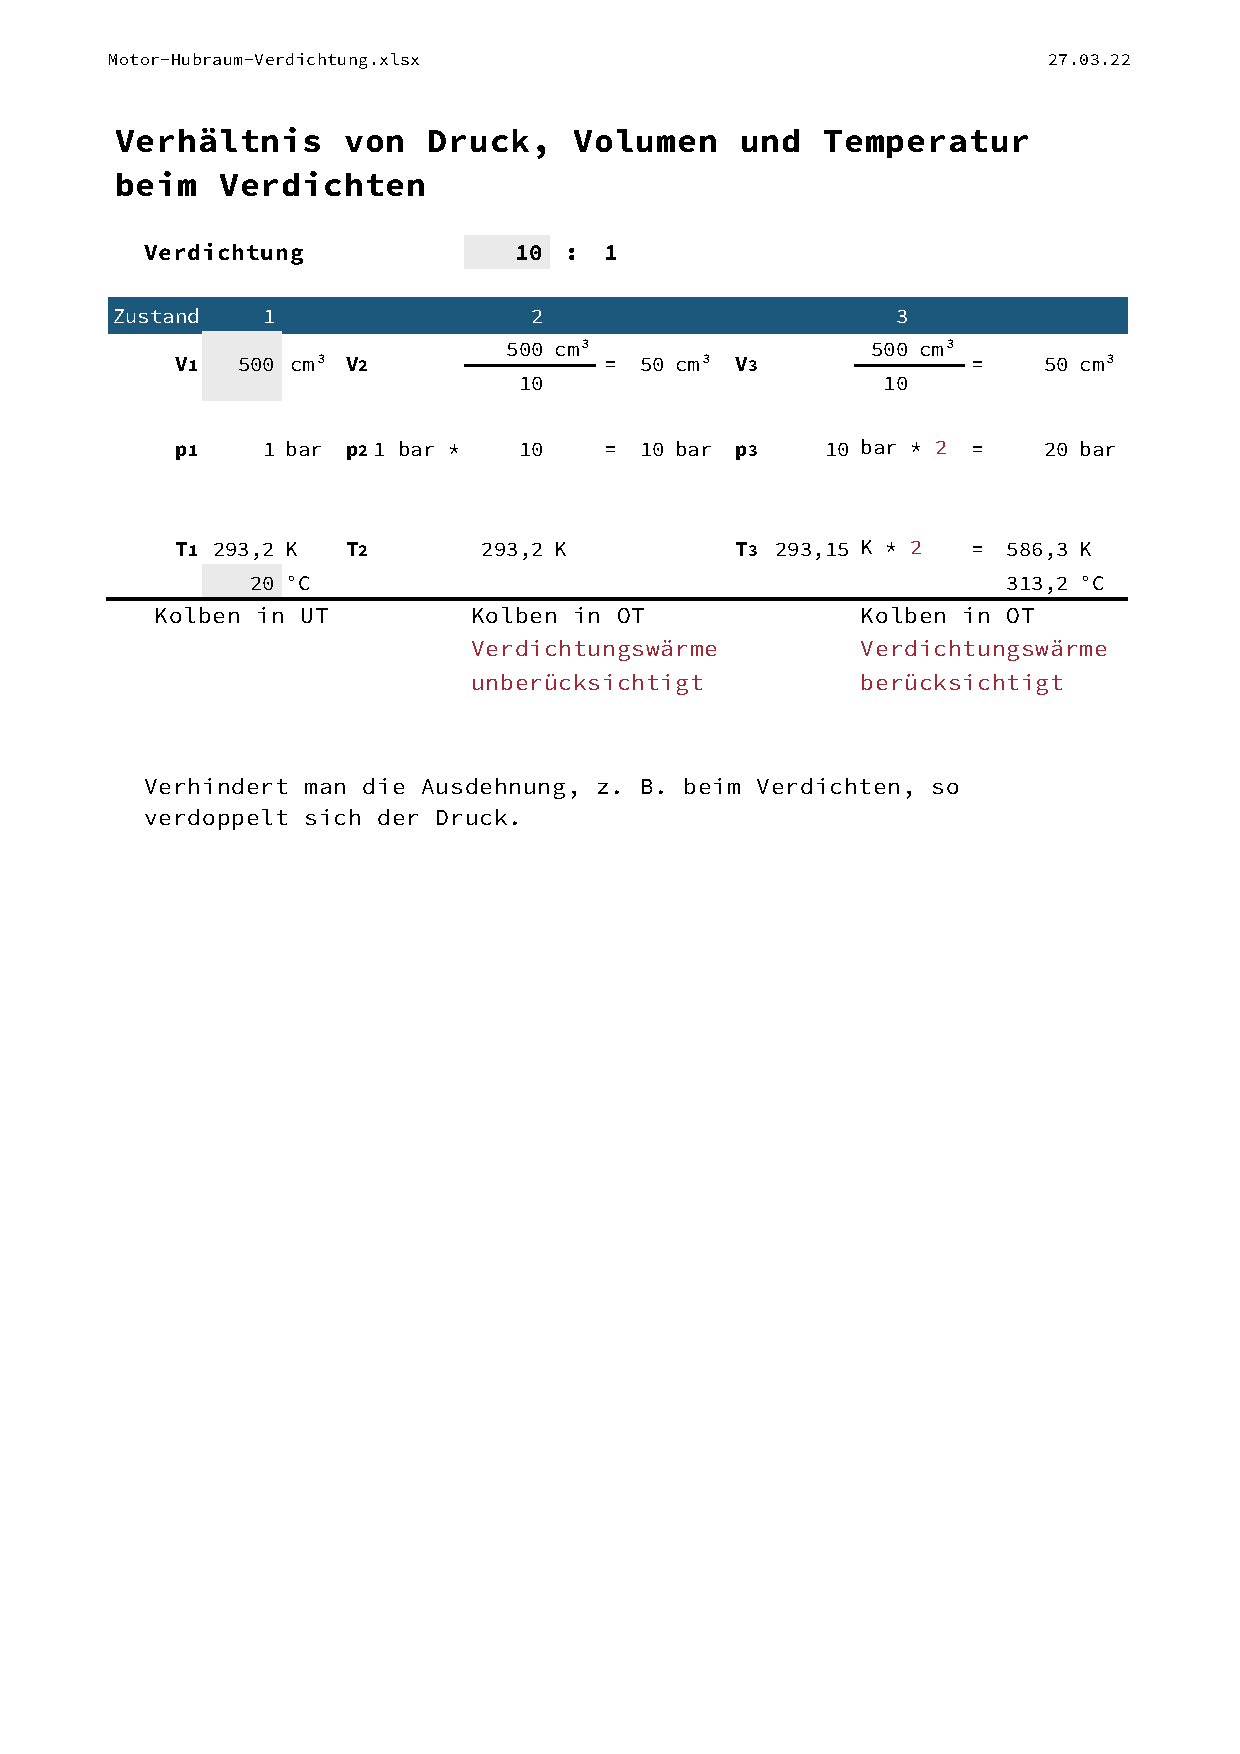
\includepdf[pages=-]{Tabellen/PDF/Druck-Volumen-Temp.pdf}

% -------
\section{Motor - Hubraum - Verdichtung}\label{sec:Motor-Hubraum-Verdichtung}\index{Motor-Hubraum-Verdichtung}
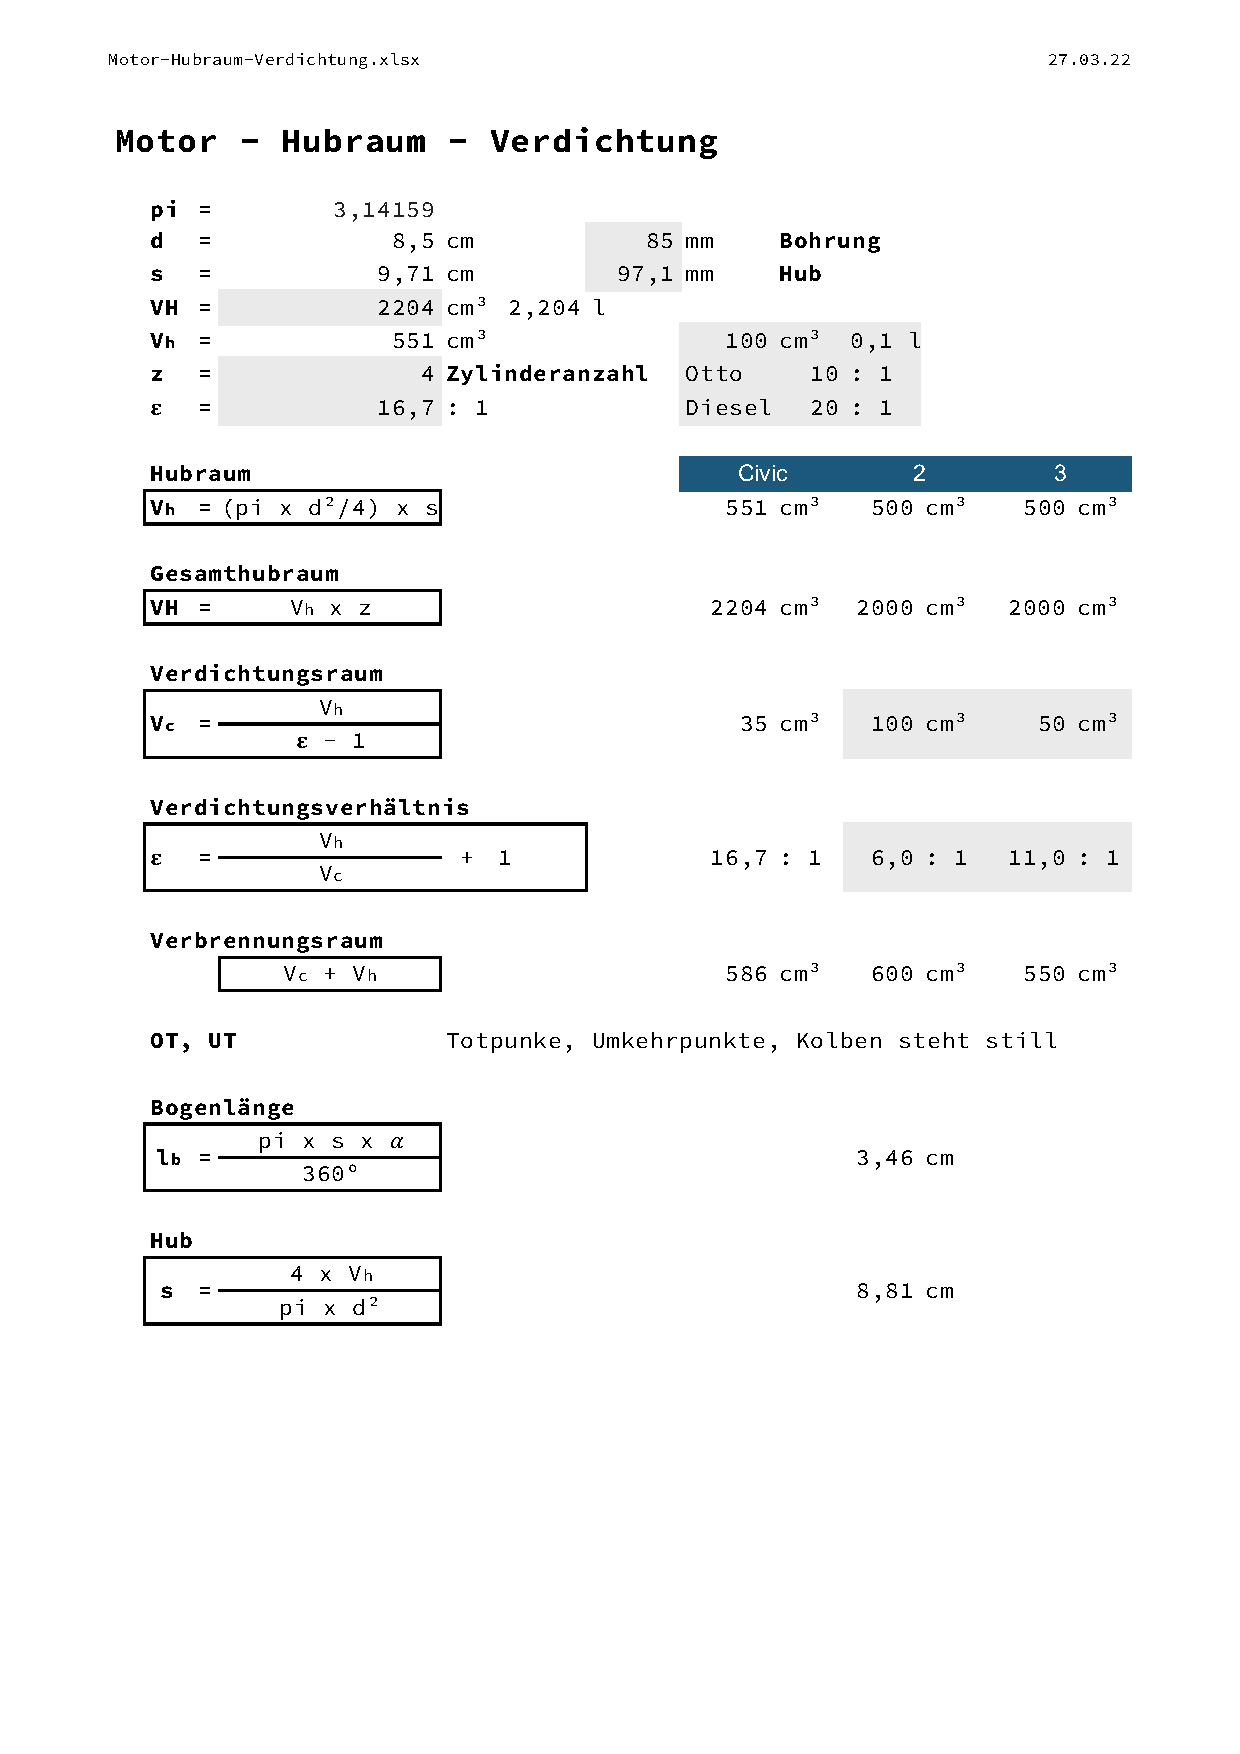
\includepdf[pages=-]{Tabellen/PDF/Motor-Hubraum-Verdichtung.pdf}





%%%%%%%%%%%%%%%%%%%%%%%%%%%%%%%%%%%%%%%%%%%%%%%%%%